% zamienne marginesy (do druku)

% \documentclass[12pt, twoside]{article}

% zwykłe marginesy (na komputer)

\documentclass[12pt]{article}
\usepackage[T1]{fontenc}
\usepackage[utf8]{inputenc}
\usepackage{graphicx} % includegraphics and all images tools
\usepackage{float}
\usepackage[intlimits]{amsmath}
\usepackage{amssymb,amsfonts}
% \usepackage{txfonts} arial 
\usepackage{fancyhdr} % Extensive control of page headers and footers
\usepackage{fancyvrb}
\usepackage{subcaption}
\usepackage{chngcntr}
\usepackage[polish]{babel}
\usepackage{polski}
\usepackage{listings}
\usepackage[hyphens]{url}
\usepackage{placeins}
\usepackage{hyperref} % links and urls in document
\usepackage{indentfirst} % wcięcie pierwszego akapitu
\usepackage{pdfpages} % include pdf in document - title page
\usepackage[figuresleft]{rotating}
\usepackage{afterpage}
\usepackage[bottom]{footmisc}

% nagłówki
%\usepackage{fancyhdr}

% podpisy nad tabelami
\floatstyle{plaintop}
\restylefloat{table}
% end

% fbox dookola bialych zdjec
\fboxsep=0mm%padding thickness
\fboxrule=0.5pt%border thickness
%end

\usepackage{makecell}

\usepackage{pifont}
\usepackage{xcolor}
\newcommand{\cmark}{\textcolor{green!80!black}{\ding{51}}}
\newcommand{\xmark}{\textcolor{red}{\ding{55}}}
\newcolumntype{L}{>{\centering\arraybackslash}m{4cm}}
\newcommand\blankpage{%
    \null
    \thispagestyle{empty}%
    \addtocounter{page}{-1}%
    \newpage}
% listingi i spis listingów
\usepackage{listings}
\usepackage{caption}

\DeclareCaptionType{code}[Listing][Spis listingów]
\lstset{language=Python,
    frame=single, % adds a frame around the code
    xleftmargin=3.4pt,
    xrightmargin=3.4pt,
    keywordstyle=\color{blue},
    basicstyle=\scriptsize\ttfamily,
    commentstyle=\color{Green}\ttfamily,
    rulecolor=\color{black},
    upquote=true,
    numbers=left,
    numberstyle=\tiny\color{gray},
    stepnumber=1,
    numbersep=8pt,
    showstringspaces=false,
    breaklines=true,
    frameround=ftff,
    frame=single,
    belowcaptionskip=1em,
    belowskip=1em,}

%linki
\hypersetup{
  colorlinks = true, %Colours links instead of ugly boxes
  urlcolor = black, %Colour for external hyperlinks
  linkcolor = black, %Colour of internal links
  citecolor = black %Colour of citations
}

\newcommand{\myparagraph}[1]{\paragraph{#1}\mbox{}\\}

\restylefloat{table}
\let\svaddcontentsline\addcontentsline
\captionsetup{justification=centering} 
\addto\captionspolish{\renewcommand{\figurename}{Rys.}}
\addto\captionspolish{\renewcommand{\tablename}{Tab.}}
\addto\captionspolish{\renewcommand{\contentsname}{Spis treści}}
\addto\captionspolish{\renewcommand{\abstractname}{}}
\addto\captionspolish{\renewcommand{\listfigurename}{Spis rysunków}}
\addto\captionspolish{\renewcommand{\listtablename}{Spis tabel}}
\renewcommand{\baselinestretch}{1.5}
\numberwithin{figure}{section}
\counterwithin{table}{section}
\counterwithin{code}{section}

\begin{document}
\begin{sloppypar}

% nazwa rozdziału w nagłówku:

% \pagestyle{fancy}
% \renewcommand{\sectionmark}[1]{\markboth{#1}{#1}}
% \renewcommand{\headrulewidth}{0pt} % Width of line at top of page
% \fancyhead[R]{\leftmark}
% \fancyhead[L]{}


% Strona tytułowa:


\includepdf{title_page.pdf}
\pagenumbering{arabic}
\setcounter{page}{2}
\setcounter{secnumdepth}{3}

% Spis treści:

\tableofcontents
\pagebreak

% Wstęp

\section{Wstęp}

Fotografia to stosunkowo nowy wynalazek --- nie minęło nawet 200 lat od wykonania pierwszego znanego nam zdjęcia, słynnego ``Widoku z okna w Le Gras'' z 1826 roku \cite{fotografia}. Początki uwieczniania obrazu przez ludzi były jednak diametralnie różne od tego, co znane jest dzisiaj. Do momentu wynalezienia matrycy światłoczułej (czyli powstania fotografii cyfrowej), rozwój technik fotograficznych polegał jedynie na ulepszaniu technologii bazującej na światłoczułości soli srebra \cite{fotografia}. Fotografia wkrótce została rozpowszechniona na całym świecie. Dało jej to ogromne znaczenie historyczne i kulturowe --- zdjęcia mogą być zarówno dziełami sztuki, jak i dokumentacją ważnych wydarzeń. Powstał również zawód fotografa, który przeszedł wiele zmian na przestrzeni czasu --- początkowo były to osoby, do których należało się udać, żeby mieć możliwość uwiecznienia swojego wizerunku. Zmiana charakterystyki wspomnianej profesji zaczęła następować wraz z wynalezieniem fotografii cyfrowej oraz rozwojem technologii informatycznych. W 1957 roku powstał pierwszy obraz cyfrowy, wykonany przez Russella Kirscha, amerykańskiego naukowca-informatyka. Był to skan analogowej fotografii jego 3-miesięcznego syna \cite{firstdigitalphoto}. Dwanaście lat później Willard S. Boyle oraz George E. Smith wynaleźli matrycę CCD\footnote{ang. CCD --- charge-coupled device.}. Z perspektywy czasu okazało się to być na tyle istotnym dokonaniem, że jego autorzy otrzymali w 2009 roku nagrodę Nobla \cite{nobelfoto}. Powstanie i rozpowszechnienie fotografii cyfrowej zbiegło się też z okresem najszybszego wzrostu ogólnej dostępności Internetu. Na przełomie tysiącleci pojawiły się media społecznościowe, w tym niektóre niemal całkowicie oparte na publikowaniu obrazów, na przykład Instagram (\url{www.instagram.com}). Ludzie codziennie dzielą się milionami zdjęć, a największe konta posiadają nawet kilkaset milionów obserwujących \cite{instagram}. Inne media społecznościowe również w dużej mierze polegają na możliwości udostępniania zdjęć. Wszystko to powoduje, że zawód fotografa jest obecnie zupełnie inny, niż w czasach przed wynalezieniem aparatu cyfrowego. Pojawiają się nowe rodzaje zleceń --- profesjonalnie wykonane zdjęcia potrzebne są nie tylko po to, aby uwiecznić przełomowe momenty w życiu człowieka lub umieścić je w prasie, ale też stanowią niezwykle ważny środek przekazu w reklamie. 

Powszechna dostępność aparatów cyfrowych oraz rozwój technologii pozwalający na polepszenie stosunku ceny do jakości sprzętu fotograficznego spowodowały jednak, że pojawiło się wielu fotografów, a co za tym idzie --- utworzyła się większa konkurencja na rynku. Trudniej jest znaleźć nowych klientów. Aby pozyskać zlecenia, w obecnych czasach konieczna jest więc odpowiednia promocja świadczonych usług. W 2022 roku kanadyjski magazyn Format przeprowadził ankietę. Brało w niej udział 3 898 fotografów z 97 krajów. Według zebranych odpowiedzi, na najważniejsze źródła pozyskiwania nowych klientów składają się polecenia od poprzednich klientów (61\% respondentów), strona internetowa z portfolio (40\%), Instagram (38\%), Facebook (25\%) oraz wyszukiwania w Google (22\%) \cite{stateofphotography}. Z danych tych wynika, że najbardziej istotnym internetowym narzędziem do pozyskiwania nowych klientów są personalne strony internetowe, na których można obejrzeć portfolio fotografa.

To, jak ma wyglądać portfolio osoby świadczącej usługi fotograficzne, w dużym stopniu zależy od tego, jaką dziedzinę fotografii reprezentuje jego właściciel. Przykładowo, fotograf ślubny oprócz samego portfolio powinien posiadać na swojej stronie internetowej dokładniejszy opis świadczonych usług, a także przydatne informacje mogące pomóc potencjalnemu klientowi podjąć decyzję o kontakcie. Osobie prowadzącej studio fotograficzne przyda się wykaz rekwizytów, a fotografowi produktowemu lista firm, z którymi współpracował. Strona tworzona w ramach tej pracy inżynierskiej będzie natomiast przeznaczona dla fotografa koncertowego i dziennikarza muzycznego. Przydatnym elementem będzie więc blog, który posłuży do umieszczania relacji z wydarzeń takich, jak koncerty czy festiwale, a także zapewni miejsce do publikowania wypowiedzi w charakterze felietonu lub recenzji.


%% Cel i założenia pracy

\subsection{Cel i założenia pracy}

Celem pracy jest zaprojektowanie oraz implementacja personalnej strony internetowej łączącej cechy strony-wizytówki, blogu z systemem komentowania oraz portfolio fotograficznego. Strona ta ma być miejscem prezentacji osiągnięć fotografa i dziennikarza muzycznego. Etap projektu skupia się na przeglądzie istniejących rozwiązań oraz na wykonaniu projektu graficznego strony. Implementacja polega na stworzeniu dwuczęściowej aplikacji sieciowej przy użyciu systemu zarządzania treścią Strapi oraz szkieletu aplikacyjnego Next.js, umożliwiającego pobieranie danych ze Strapi oraz renderowanie treści po stronie serwera, co pozwala na korzystne pozycjonowanie strony w wyszukiwarkach internetowych. 

%% Układ pracy

\subsection{Układ pracy}

Rozdział pierwszy wprowadza do tematyki oraz problematyki pracy. Drugi rozdział jest przeglądem istniejących rozwiązań --- personalnych stron-wizytówek popularnych zagranicznych fotografów koncertowych, portali społecznościowych używanych w branży, a także blogów i innych stron o tematyce muzycznej. W rozdziale trzecim przedstawione są narzędzia, które zostały wykorzystane podczas projektowania oraz implementacji tworzonej strony internetowej. Rozdział czwarty poświęcony jest projektowi portfolio i blogu --- znalazły się w nim założenia projektu, wymagania funkcjonalne i niefunkcjonalne oraz opis realizacji projektu. Piąty rozdział jest prezentacją wykonanej strony internetowej, a szósty podsumowuje realizację projektu, celu oraz założeń pracy.

% Przegląd istniejących rozwiązań 

\newpage

\section{Przegląd istniejących rozwiązań}

Fotografia i dziennikarstwo to branże, które wzajemnie od siebie zależą. Zdjęcia urozmaicają relacje prasowe z wydarzeń, powodują, że artykuły są ciekawsze, a odbiór fotoreportażu jest lepszy wtedy, gdy przedstawiona jest jakaś historia. Aby strona internetowa realizowana na potrzeby tej pracy inżynierskiej była wykonana z zachowaniem najlepszych możliwych praktyk, został przeprowadzony przegląd istniejących rozwiązań posiadających podobne funkcje. Pozwoli to na znalezienie inspiracji, wyciągnięcie wniosków i wykorzystanie ich zarówno podczas projektowania wyglądu strony, jak i na etapie implementacji.

%% Personalne strony-wizytówki fotografów

\subsection{Personalne strony-wizytówki fotografów}

Personalne strony-wizytówki fotografów są zazwyczaj nieskomplikowane pod względem budowy, nawigacji oraz wyglądu. Rozkład elementów powinien być możliwie prosty, żeby potencjalny klient oglądający portfolio mógł skupić się na jego zawartości. W tym podrozdziale zostaną poddane analizie dwie strony profesjonalnych fotografów działających w branży muzycznej.

%%% Ashley Osborn

\subsubsection{Ashley Osborn} \label{ashley}

Ashley Osborn jest amerykańską fotografką zamieszkałą w Los Angeles. Specjalizuje się w dokumentowaniu tras koncertowych, ale zajmuje się też wykonywaniem sesji zdjęciowych oraz tworzeniem teledysków. Współpracowała z najpopularniejszymi artystami muzycznymi z całego świata oraz globalnymi firmami z branży kulturowej \cite{ashley}. 

\begin{figure}[H] 
    \centering
         \fbox{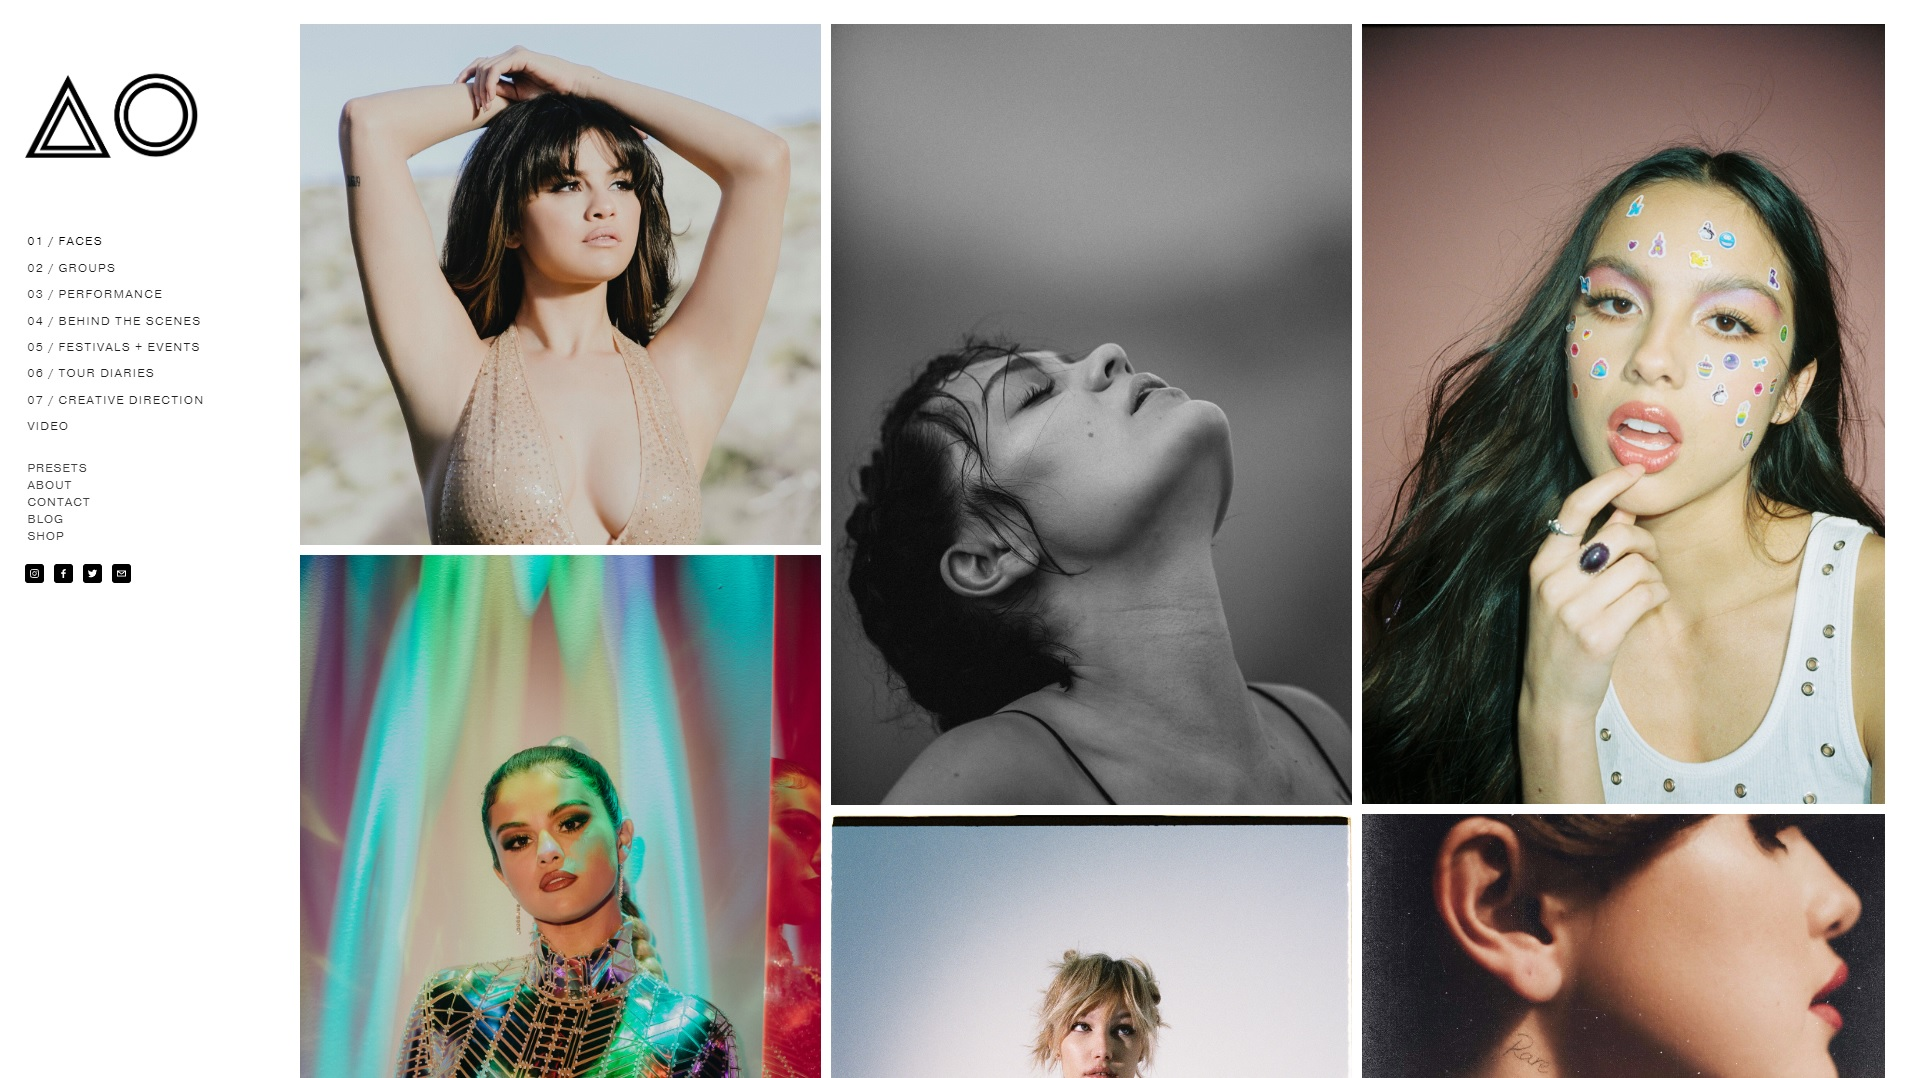
\includegraphics[width=0.99\textwidth]{images/ashley-1.jpg}}
   \caption{\textit{\url{www.ashleyosborn.com}} --- strona główna.}
   \label{fig:ashley-1.jpg}
\end{figure}

Rysunek \ref{fig:ashley-1.jpg} przedstawia wygląd strony głównej witryny internetowej \url{www.ashleyosborn.com}. Warto zwrócić szczególną uwagę na kilka jej elementów. W lewym górnym rogu znajduje się logo będące inicjałami właścicielki analizowanej strony. Pełni ono funkcję estetyczną i jest ważną częścią identyfikacji wizualnej. Ponadto, będąc w dowolnym miejscu na stronie fotografki, można na nie kliknąć --- spowoduje to przeniesienie użytkownika na stronę główną. Oprócz logo, w lewej części strony umieszczone zostało menu, które też jest zawsze widoczne. Resztę, a zarazem większość ekranu, wypełniają zdjęcia. Warto zaznaczyć, że ich wybór nie jest przypadkowy --- osoby, które się na nich pojawiły, są znanymi na świecie artystkami. Przykładowo osoba pozująca na pierwszej fotografii od lewej to Selena Gomez - posiada ona największą liczbę (ponad 373 miliony) obserwujących na Instagramie \cite{instagram}. 

\begin{figure}[H] 
    \centering
         \fbox{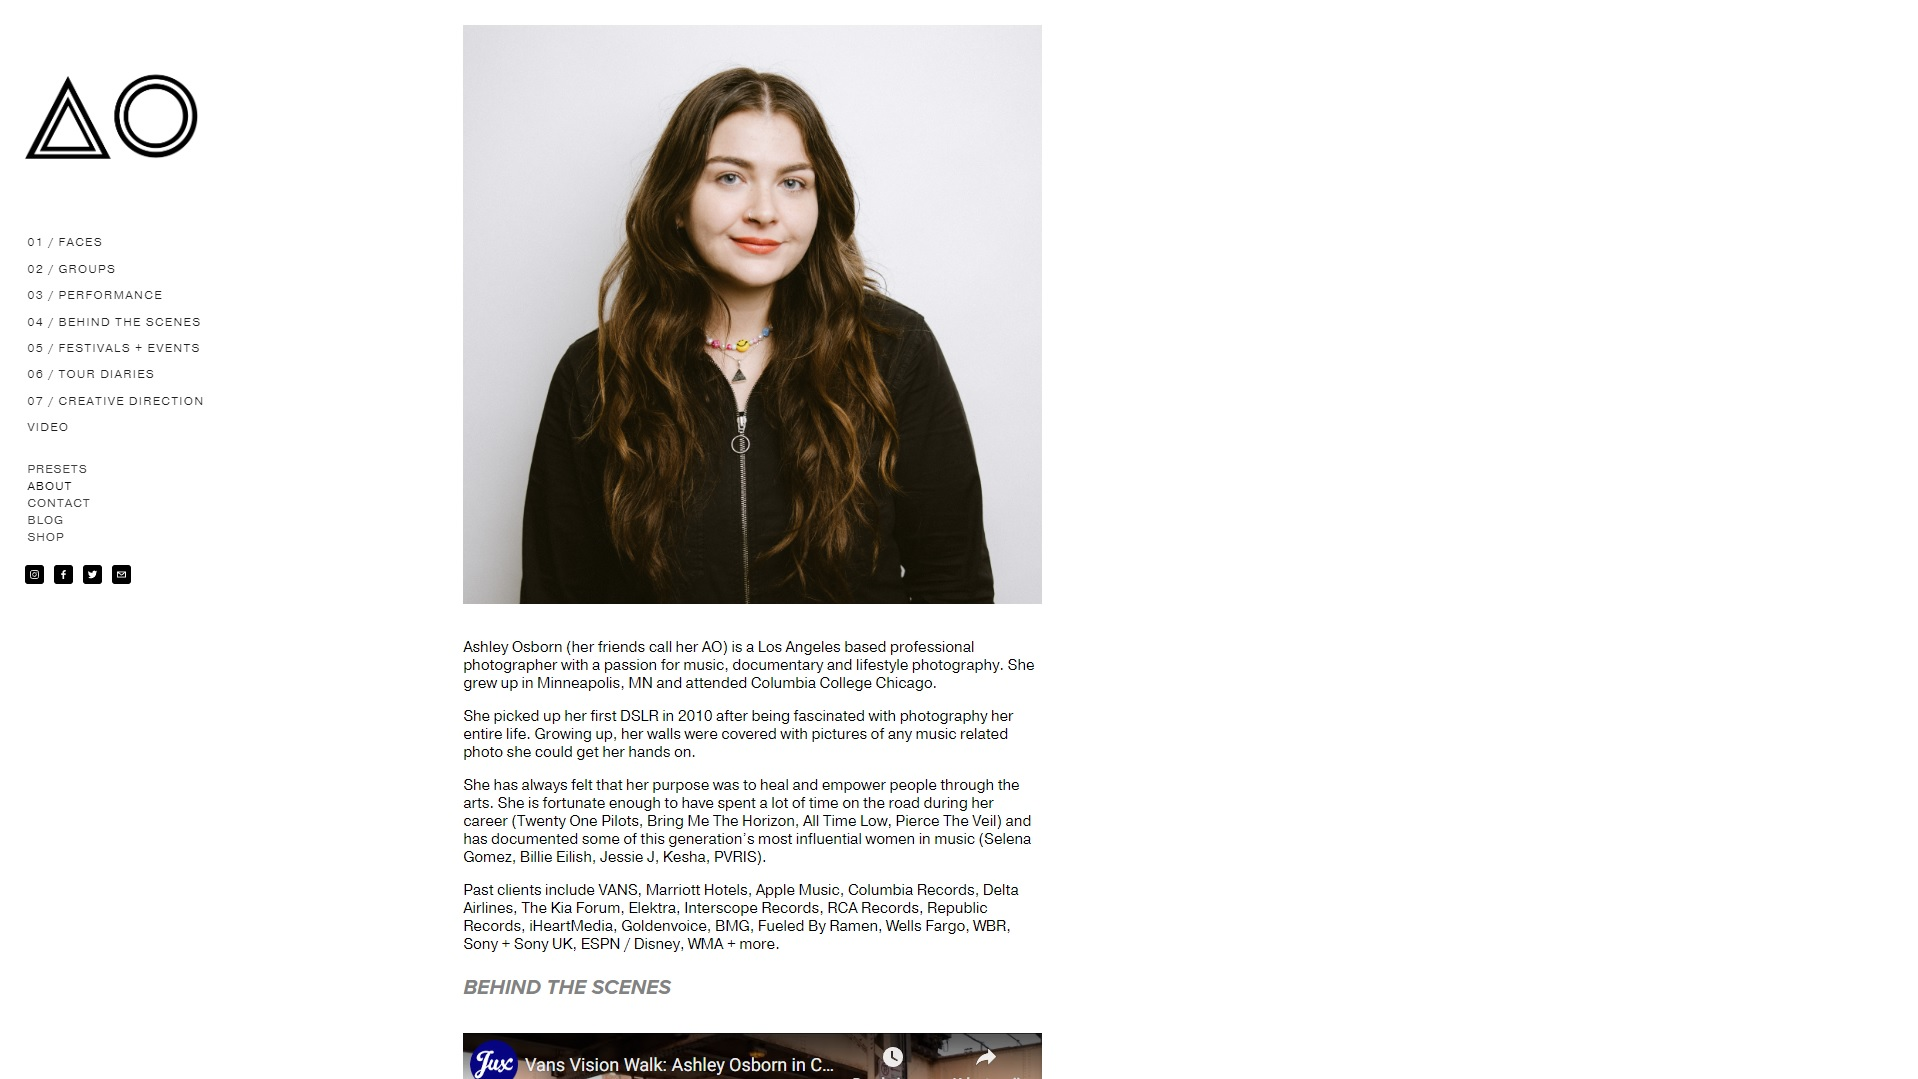
\includegraphics[width=0.99\textwidth]{images/ashley-2.jpg}}
   \caption{\textit{\url{www.ashleyosborn.com}} --- sekcja ``o mnie''.}
   \label{fig:ashley-2.jpg}
\end{figure}

\begin{figure}[H] 
    \centering
         \fbox{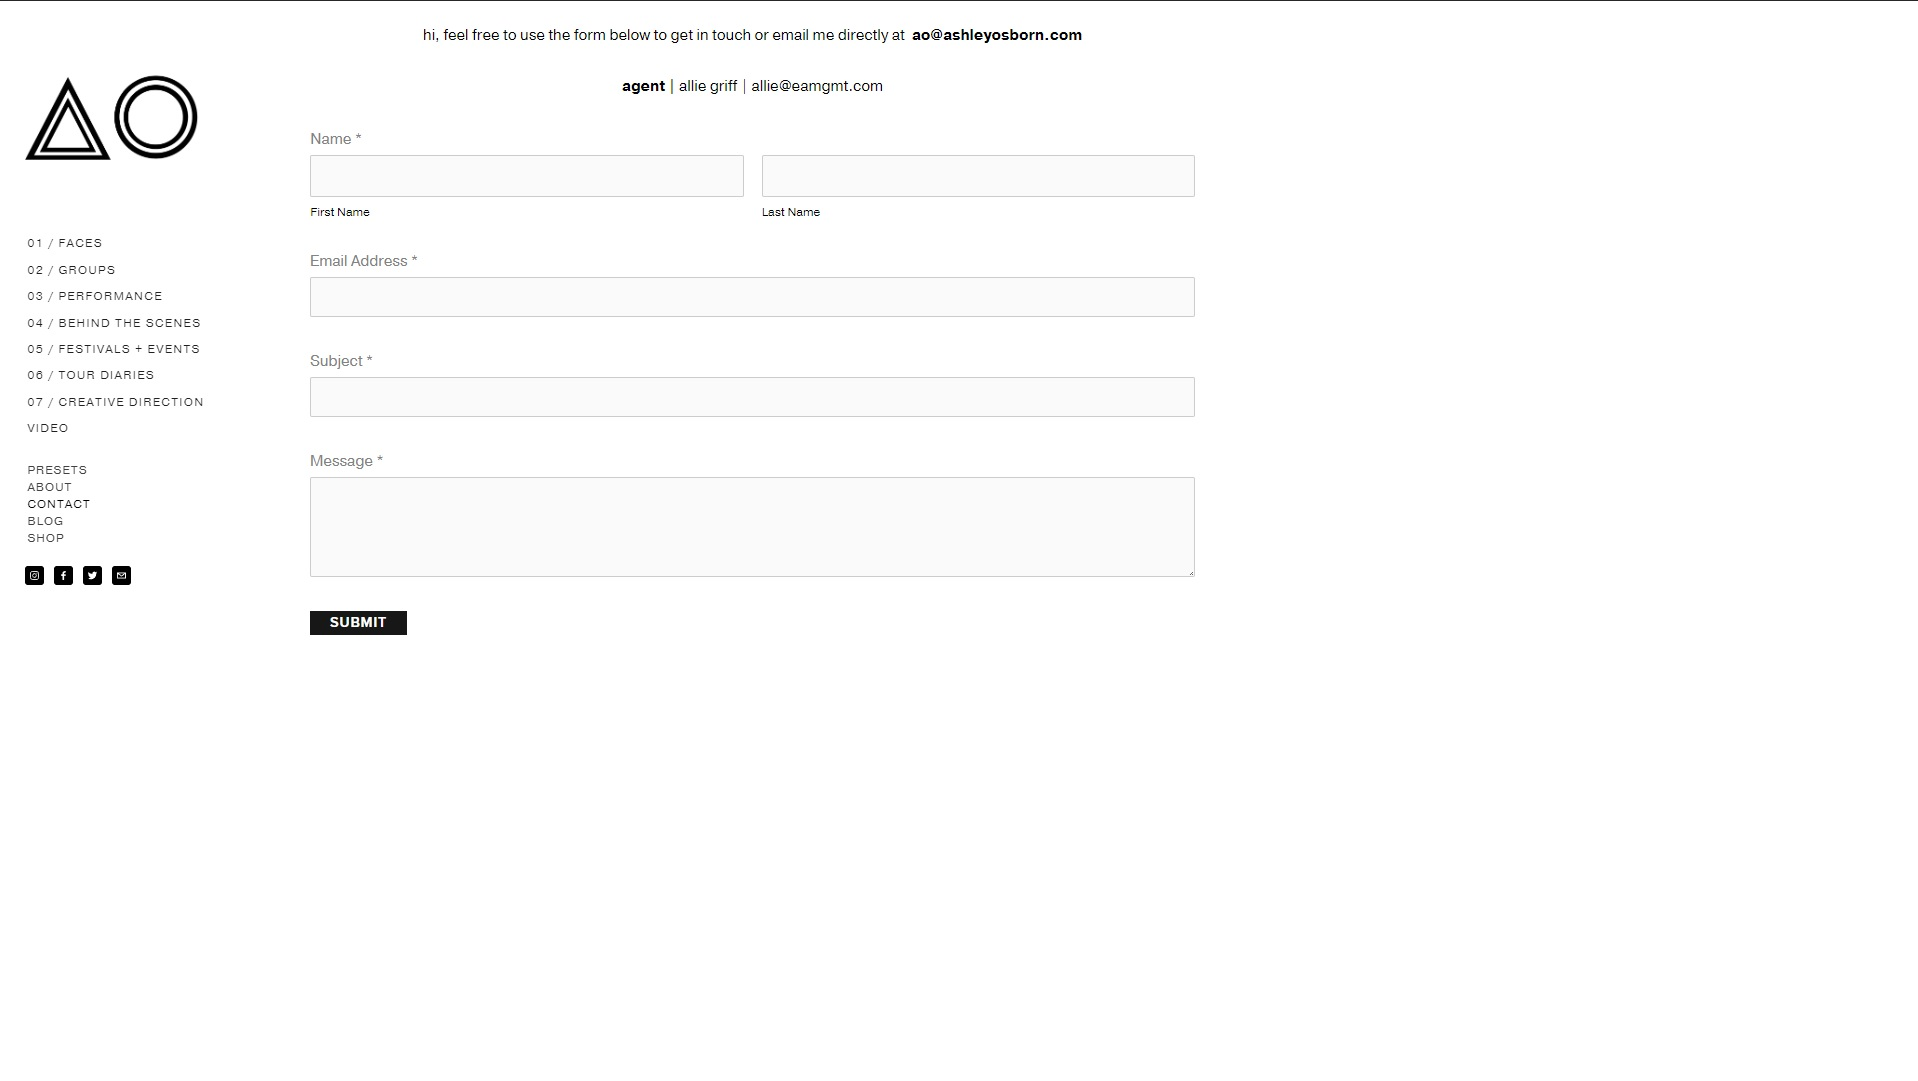
\includegraphics[width=0.99\textwidth]{images/ashley-3.jpg}}
   \caption{\textit{\url{www.ashleyosborn.com}} --- formularz kontaktowy.}
   \label{fig:ashley-3.jpg}
\end{figure}

\newpage

Widoczna na rysunku \ref{fig:ashley-2.jpg} sekcja ``o mnie'' jest kolejnym nieodłącznym elementem każdej strony-wizytówki należącej do osoby zajmującej się profesjonalną fotografią. Pozwala ona przedstawić wygląd, charakter i osiągnięcia osoby, która chce zachęcić potencjalnych klientów do skorzystania z usługi. Nie musi być ona rozbudowana --- w tym przypadku są to portret oraz krótki, lecz treściwy opis życiorysu Ashley Osborn. Zawiera on między innymi wykaz najważniejszych zleceń z przeszłości, nazwę ukończonej szkoły wyższej, a także obecne miejsce zamieszkania. Formularz kontaktowy z rysunku \ref{fig:ashley-3.jpg} umożliwia szybkie wysłanie wiadomości bez konieczności używania poczty elektronicznej lub mediów społecznościowych. Warto zwrócić uwagę na gwiazdki przy polach obowiązkowych (w tym przypadku --- po prostu wszystkich polach). Wprowadzane dane powinny być walidowane, a użytkownik poinformowany zarówno wtedy, gdy próba wysłania danych powiedzie się, jak i wtedy, gdy wystąpi błąd \cite{formularze}. 

Ostatnią sekcją strony Ashley Osborn jest blog, skonstruowany w prosty sposób, podobny do reszty strony. Użytkownik może wybrać interesujący go post z listy (rys. \ref{fig:ashley-4.jpg}), po czym przenoszony jest do jego treści (rys. \ref{fig:ashley-5.jpg}). Należy tu się przyjrzeć tekstowi --- nie zajmuje on całej szerokości strony. Ułatwia to czytanie - zarówno zbyt szerokie, jak i zbyt wąskie akapity skutecznie zniechęcają użytkownika do czytania \cite{szerokosc}. Oprócz rzeczy przedstawionych na powyższych zrzutach ekranu, na stronie istnieje też możliwość przejścia do sklepu, w którym sprzedawane są \textit{presety}\footnote{ang. preset --- zestaw gotowych ustawień, najczęściej wykorzystywany przy obróbce dużej liczby zdjęć, pozwalający na utrzymanie spójnej stylistyki na każdym z nich.} do programu do obróbki zdjęć Adobe Lightroom.

\begin{figure}[H] 
    \centering
         \fbox{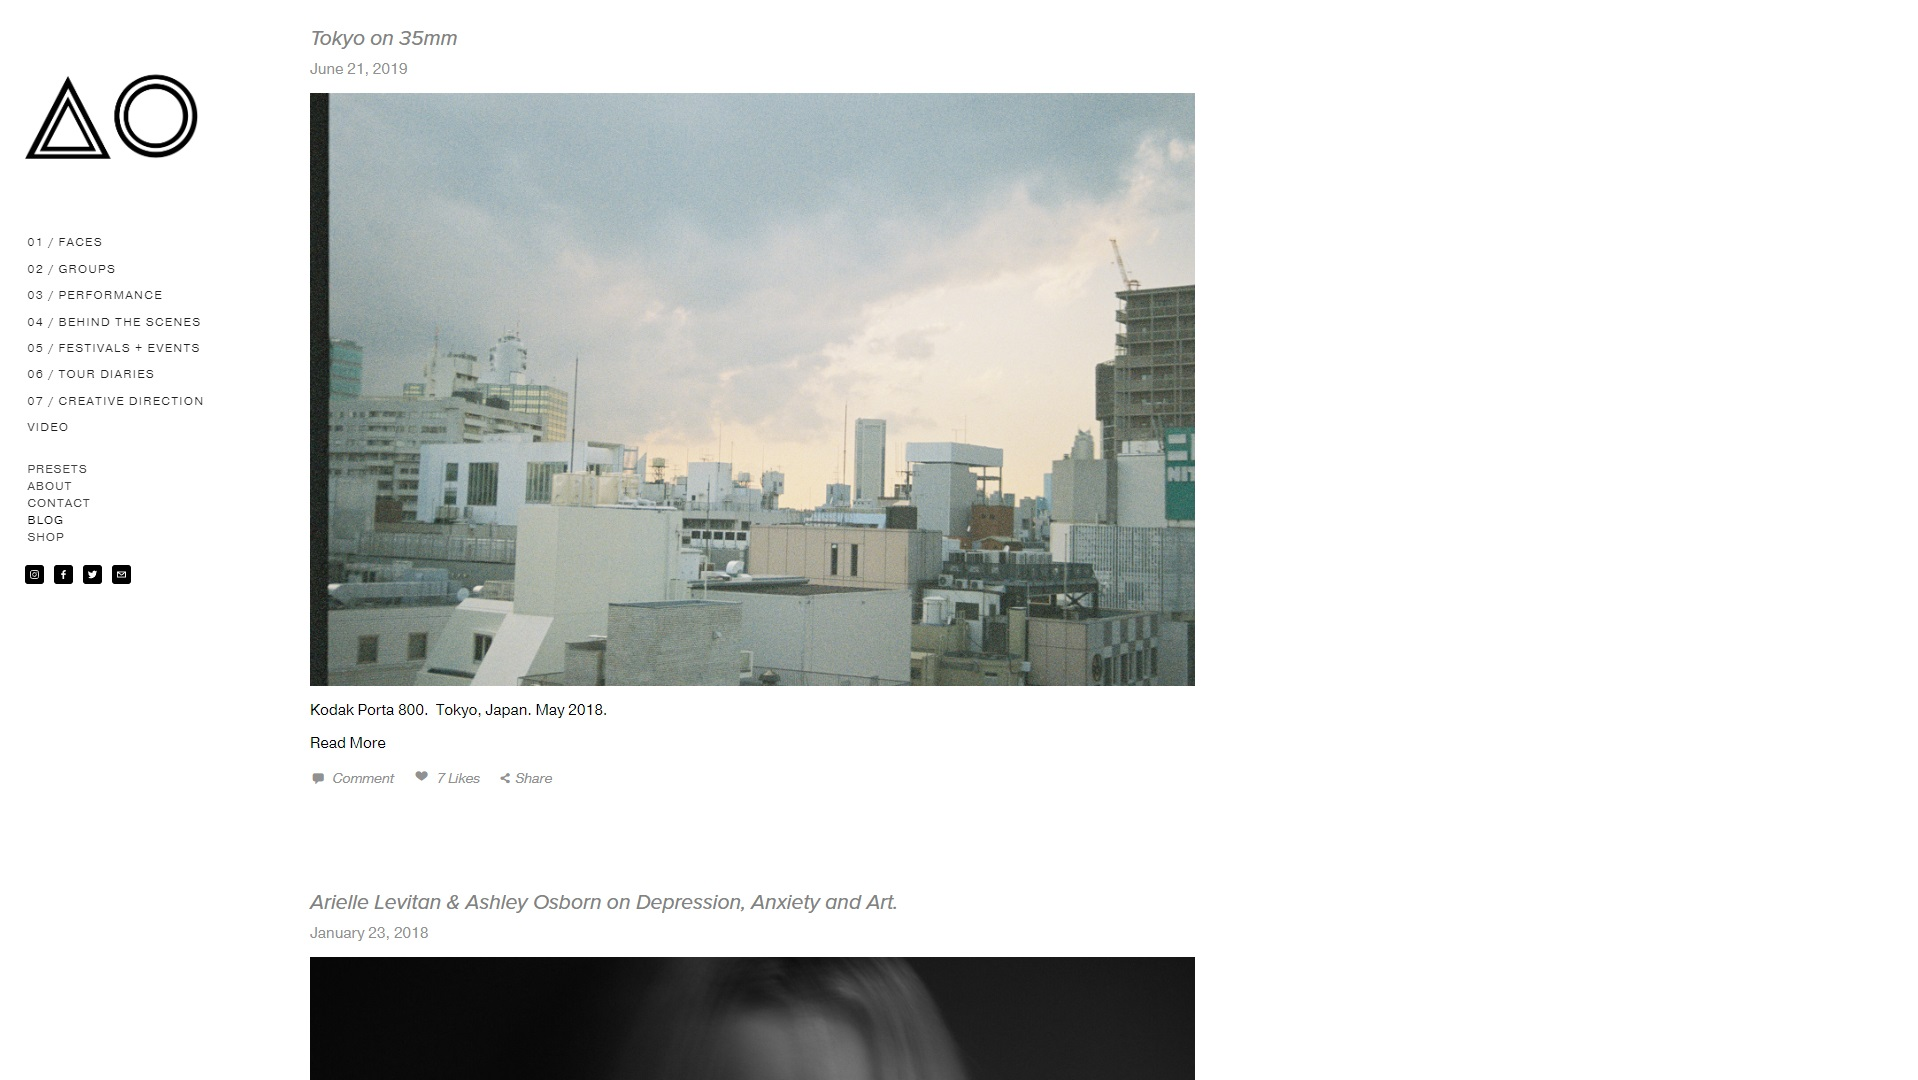
\includegraphics[width=0.99\textwidth]{images/ashley-4.jpg}}
   \caption{\textit{\url{www.ashleyosborn.com}} --- blog (lista postów).}
   \label{fig:ashley-4.jpg}
\end{figure}

\begin{figure}[H] 
    \centering
         \fbox{
\includegraphics[width=0.99\textwidth]{images/ashley-5.jpg}}
   \caption{\textit{\url{www.ashleyosborn.com}} --- blog (widok postu).}
   \label{fig:ashley-5.jpg}
\end{figure}


%%% Zackery Michael

\newpage

\subsubsection{Zackery Michael}

\begin{figure}[H] 
    \centering
         \fbox{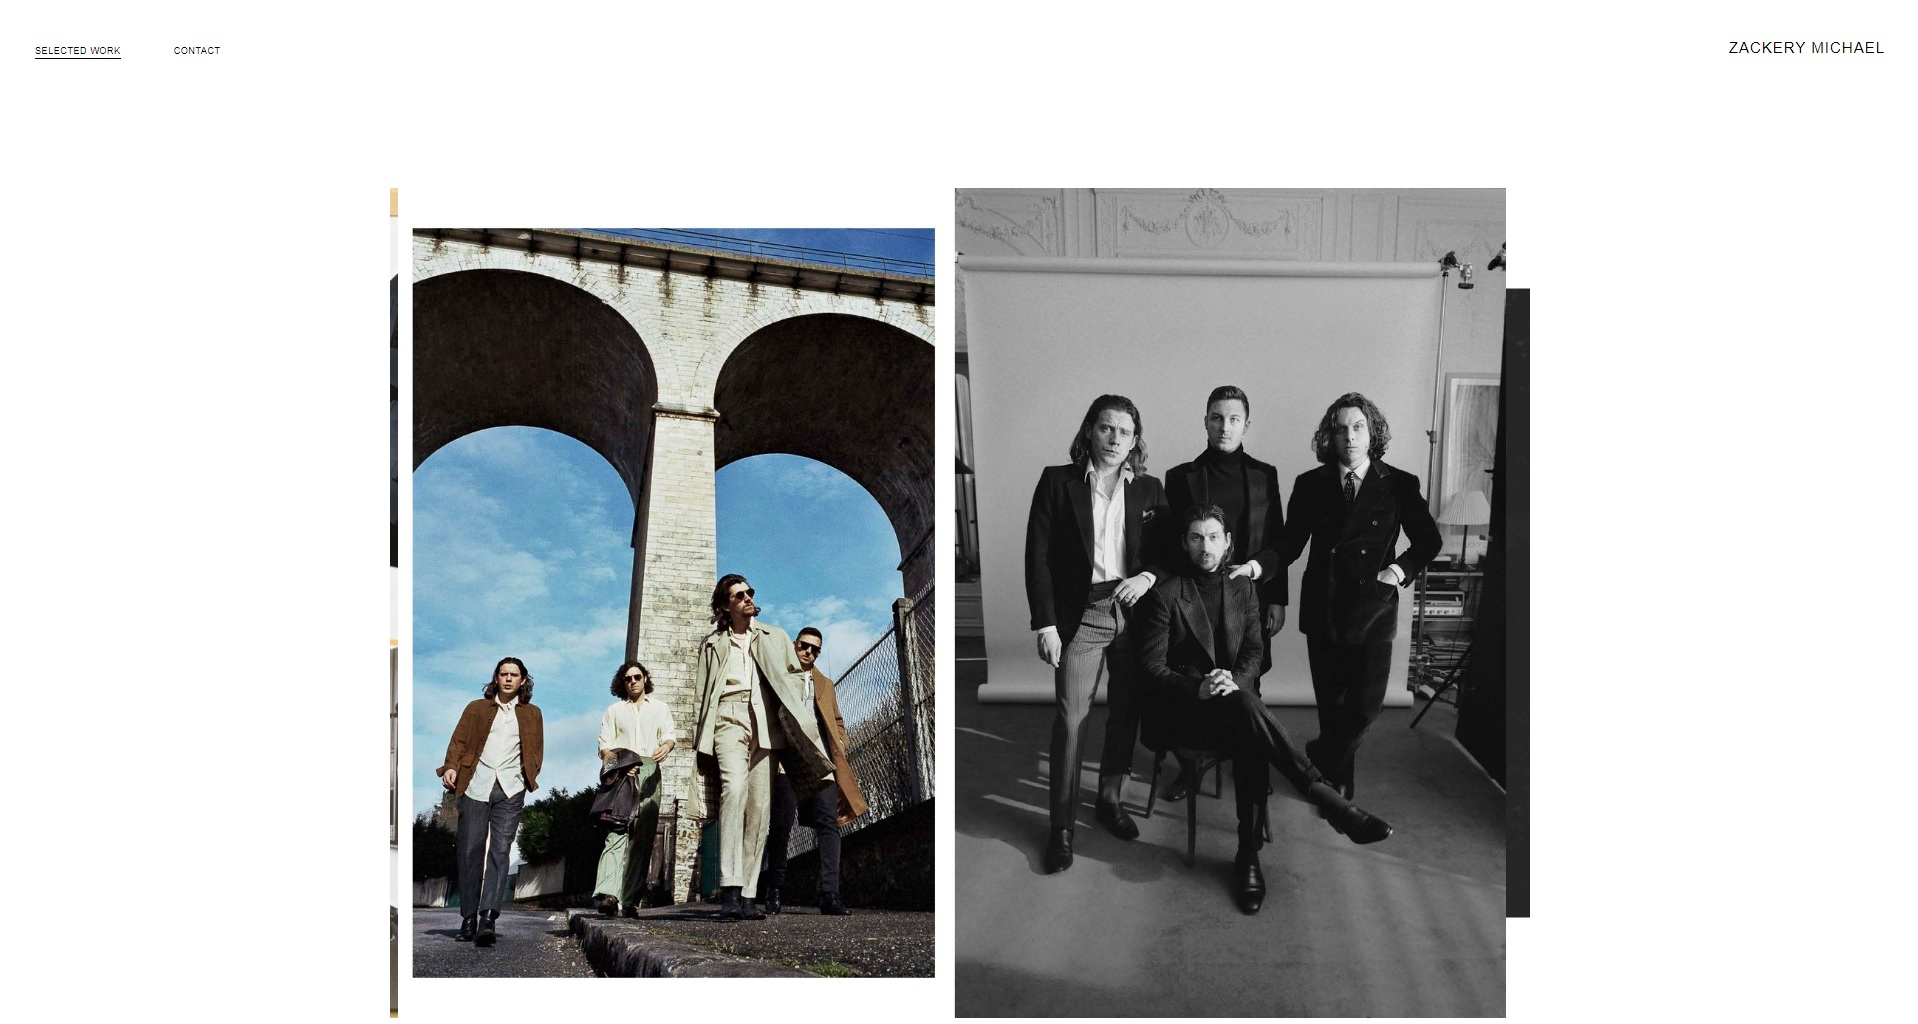
\includegraphics[width=0.99\textwidth]{images/zackery-1.jpg}}
   \caption{\textit{\url{www.zackerymichaelstudio.com}} --- strona główna.}
   \label{fig:zackery-1.jpg}
\end{figure}

\begin{figure}[H] 
    \centering
         \fbox{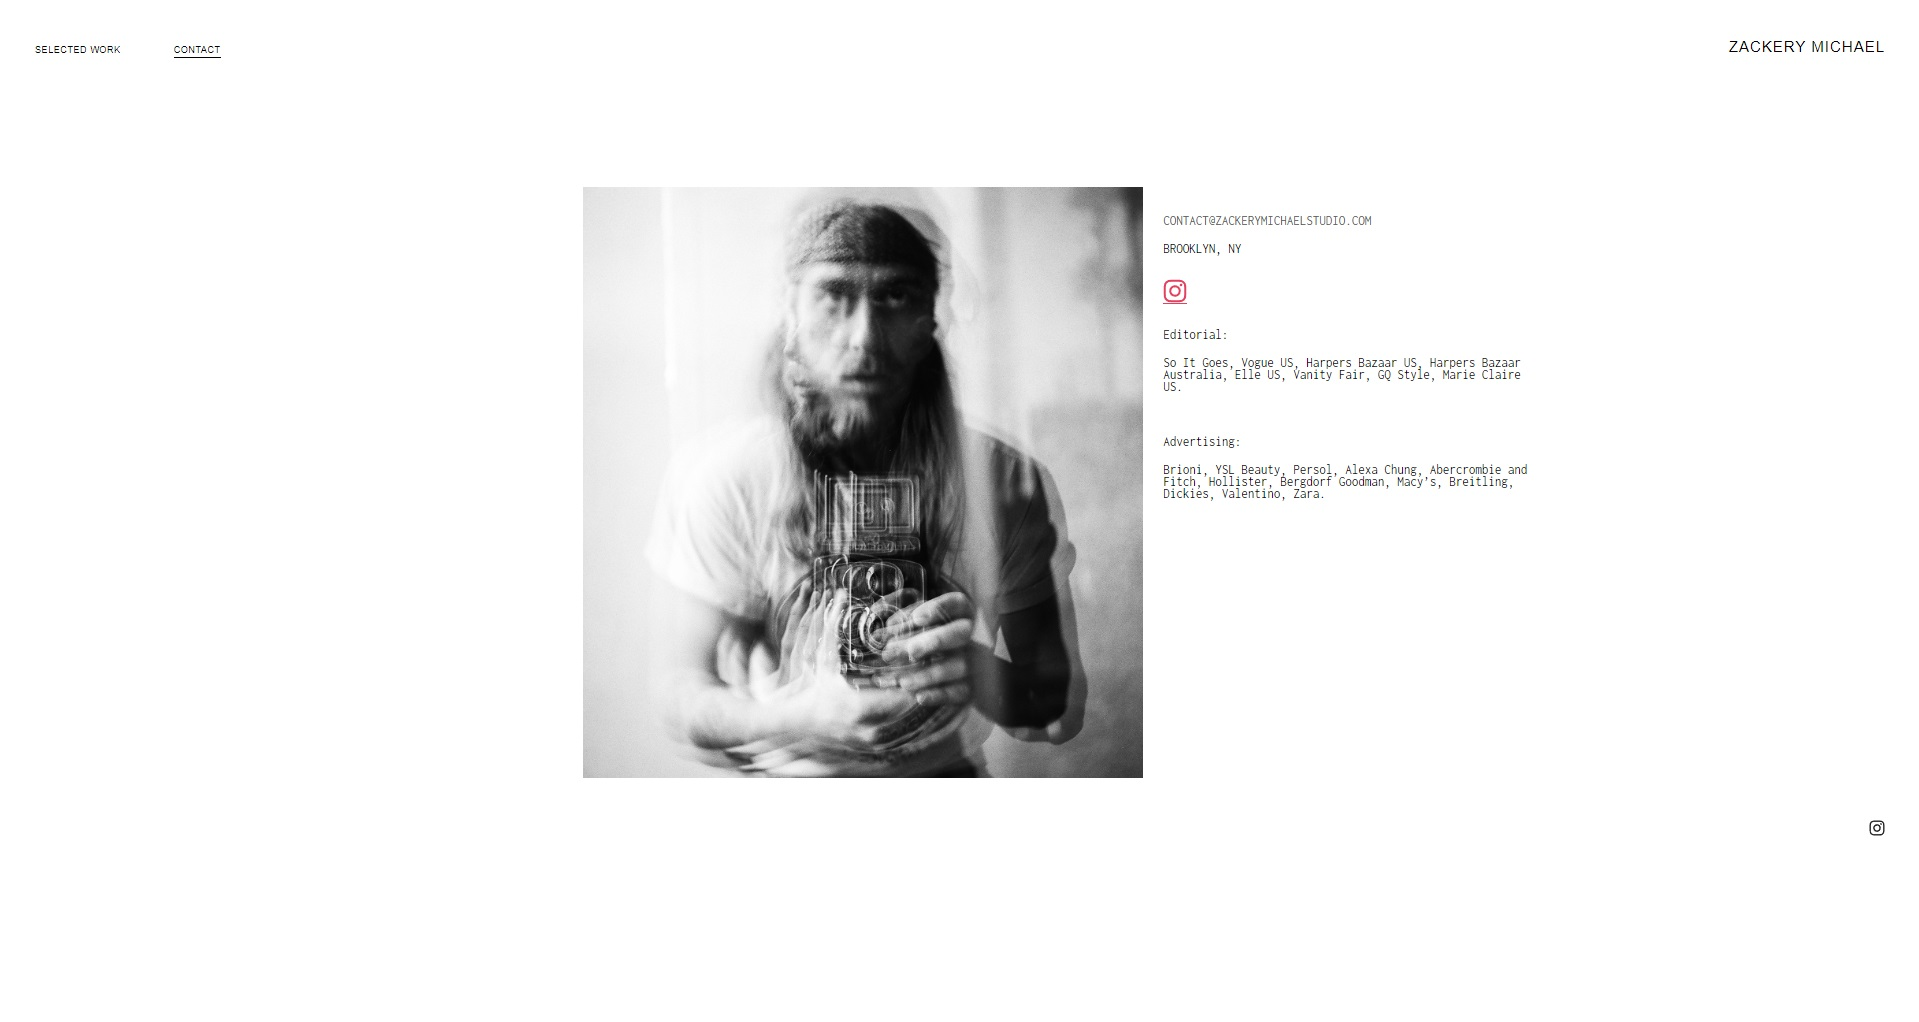
\includegraphics[width=0.99\textwidth]{images/zackery-2.jpg}}
   \caption{\textit{\url{www.zackerymichaelstudio.com}} --- sekcja kontaktowa.}
   \label{fig:zackery-2.jpg}
\end{figure}

Druga przedstawiona strona-wizytówka jest zupełnie inna w porównaniu do poprzedniej. O ile sam wygląd pierwszej analizowanej witryny był prosty, to ilość treści była dość bogata (blog, sekcja ``o mnie'', oddzielny formularz kontaktowy czy nawet sklep). W przypadku portfolio nowojorskiego fotografa Zackery'ego Michaela zastosowano zdecydowanie bardziej minimalistyczne podejście. Jego witryna internetowa składa się jedynie z dwóch części: strony głównej, przeznaczonej do zaprezentowania wybranych prac (rys. \ref{fig:zackery-1.jpg}) oraz sekcji ``kontakt'', gdzie obok zdjęcia przedstawiającego Zackery'ego Michaela podany jest jego adres poczty elektronicznej oraz przedstawione są najważniejsze firmy, z którymi współpracował fotograf (rys. \ref{fig:zackery-2.jpg}). Tekst jest znacznie ograniczony w celu zwrócenia pełnej uwagi odwiedzających stronę na prace zaprezentowane przez Zackery'ego Michaela.

%% Portale społecznościowe

\subsection{Portale społecznościowe}

Wraz z rozwojem technologii internetowych pojawiły się portale społecznościowe, które w dzisiejszych czasach mają ogromne znaczenie zarówno w znaczeniu społecznym (ułatwiają kontakt oraz zawieranie nowych znajomości przez Internet), jak i biznesowym (ze względu na wielką popularność są potężnym narzędziem marketingowym i źródłem pozyskiwania klientów). W kontekście zawodu fotografa są one o tyle ważne, że Instagram oraz Facebook, czyli te najbardziej popularne, są w dużej mierze oparte na udostępnianiu zdjęć. Pomaga to w budowaniu marki osobistej osoby świadczącej usługi fotograficzne, co ułatwia zdobywanie nowych zleceń i poszerzanie działalności poza rynek lokalny \cite{socialmedia}. Wspomniane portale społecznościwe zostaną w tym rozdziale opisane pod kątem prezentacji treści, zwłaszcza postów (Facebook) i zdjęć (Instagram) oraz profilów użytkownika.

%%% Instagram

\subsubsection{Instagram}

Instagram to powstały w 2010 roku \cite{instagramfirstday} portal społecznościowy skupiony na możliwości udostępniania zdjęć i filmów, które następnie mogą być polubione\footnote{polubienie, potocznie lajk (ang. like) --- wyrażenie aprobaty wobec treści poprzez np. kliknęcie kciuka w górę lub symbolu serca.} oraz komentowane przez innych użytkowników. Wśród fotografów jego popularność jest szczególnie duża ze względu na możliwość pełnienia przez ten serwis funkcji portfolio oraz łatwość podjęcia kontaktu poprzez wiadomości bezpośrednie. Przykładowym zaprezentowanym profilem użytkownika będzie widoczny na rysunku \ref{fig:instagram-1.jpg} profil Ashley Osborn, fotografki, której strona internetowa została opisana w podrozdziale \ref{ashley}. Składa się on z kilku elementów, którymi są: 
\begin{itemize}
    \item Część nagłówkowa ze zdjęciem profilowym, informacjami o liczbie postów, osób obserwujących oraz obserwowanych, opisem profilu oraz linkiem do strony internetowej.
    \item Zapisane relacje (ang. \textit{stories} --- wprowadzony w 2016 roku mechanizm Instagrama, pozwalający na udostępnianie zdjęć oraz filmów znikających po 24 godzinach \cite{stories}).
    \item Galeria w postaci szerokiej na trzy elementy siatki kwadratowych zdjęć lub filmów. Warto zwrócić uwagę, że trzy pierwsze posty są przypięte, a kolejne --- ułożone w kolejności od najnowszych do najstarszych. Opcja przypinania postów daje użytkownikom większy wpływ na wygląd ich profilu poprzez wyróżnienie ulubionych zdjęć lub filmów.
\end{itemize}

\begin{figure}[H] 
    \centering
         \fbox{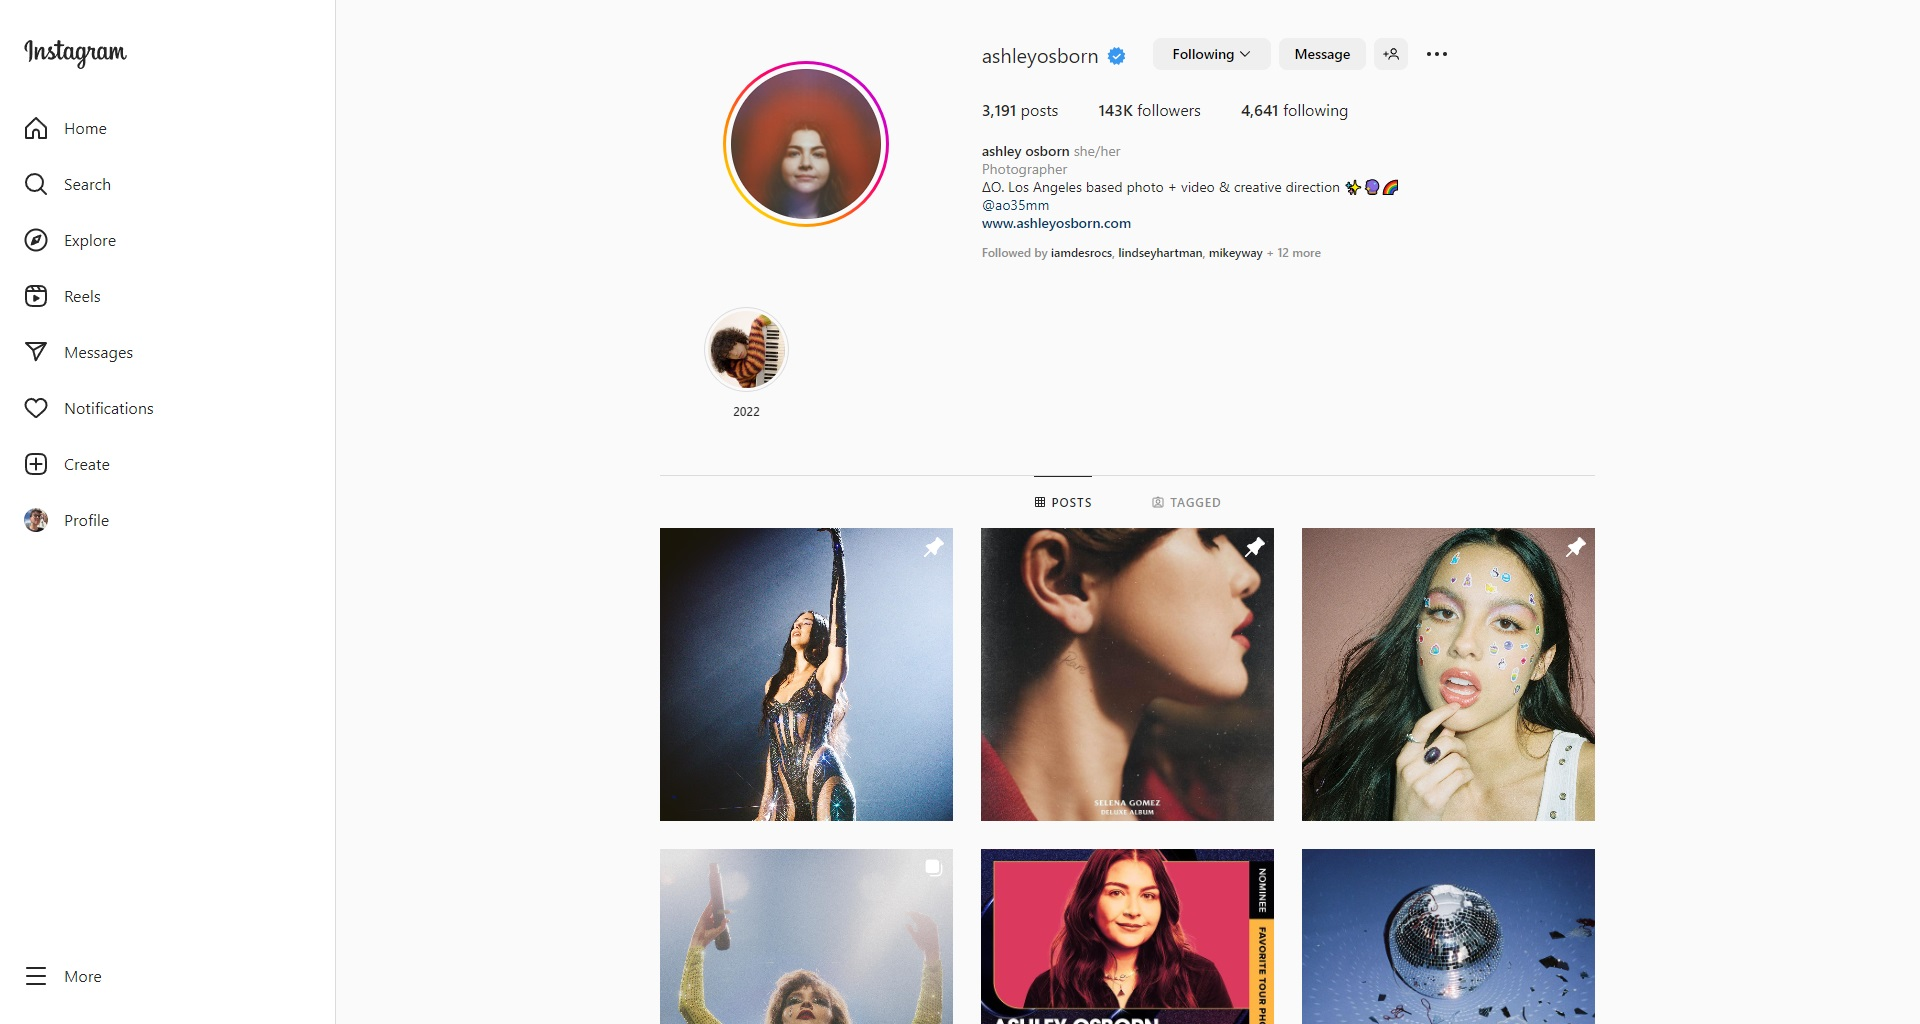
\includegraphics[width=0.99\textwidth]{images/instagram-1.jpg}}
   \caption{Instagram --- profil użytkownika.}
   \label{fig:instagram-1.jpg}
\end{figure}

\begin{figure}[H] 
    \centering
         \fbox{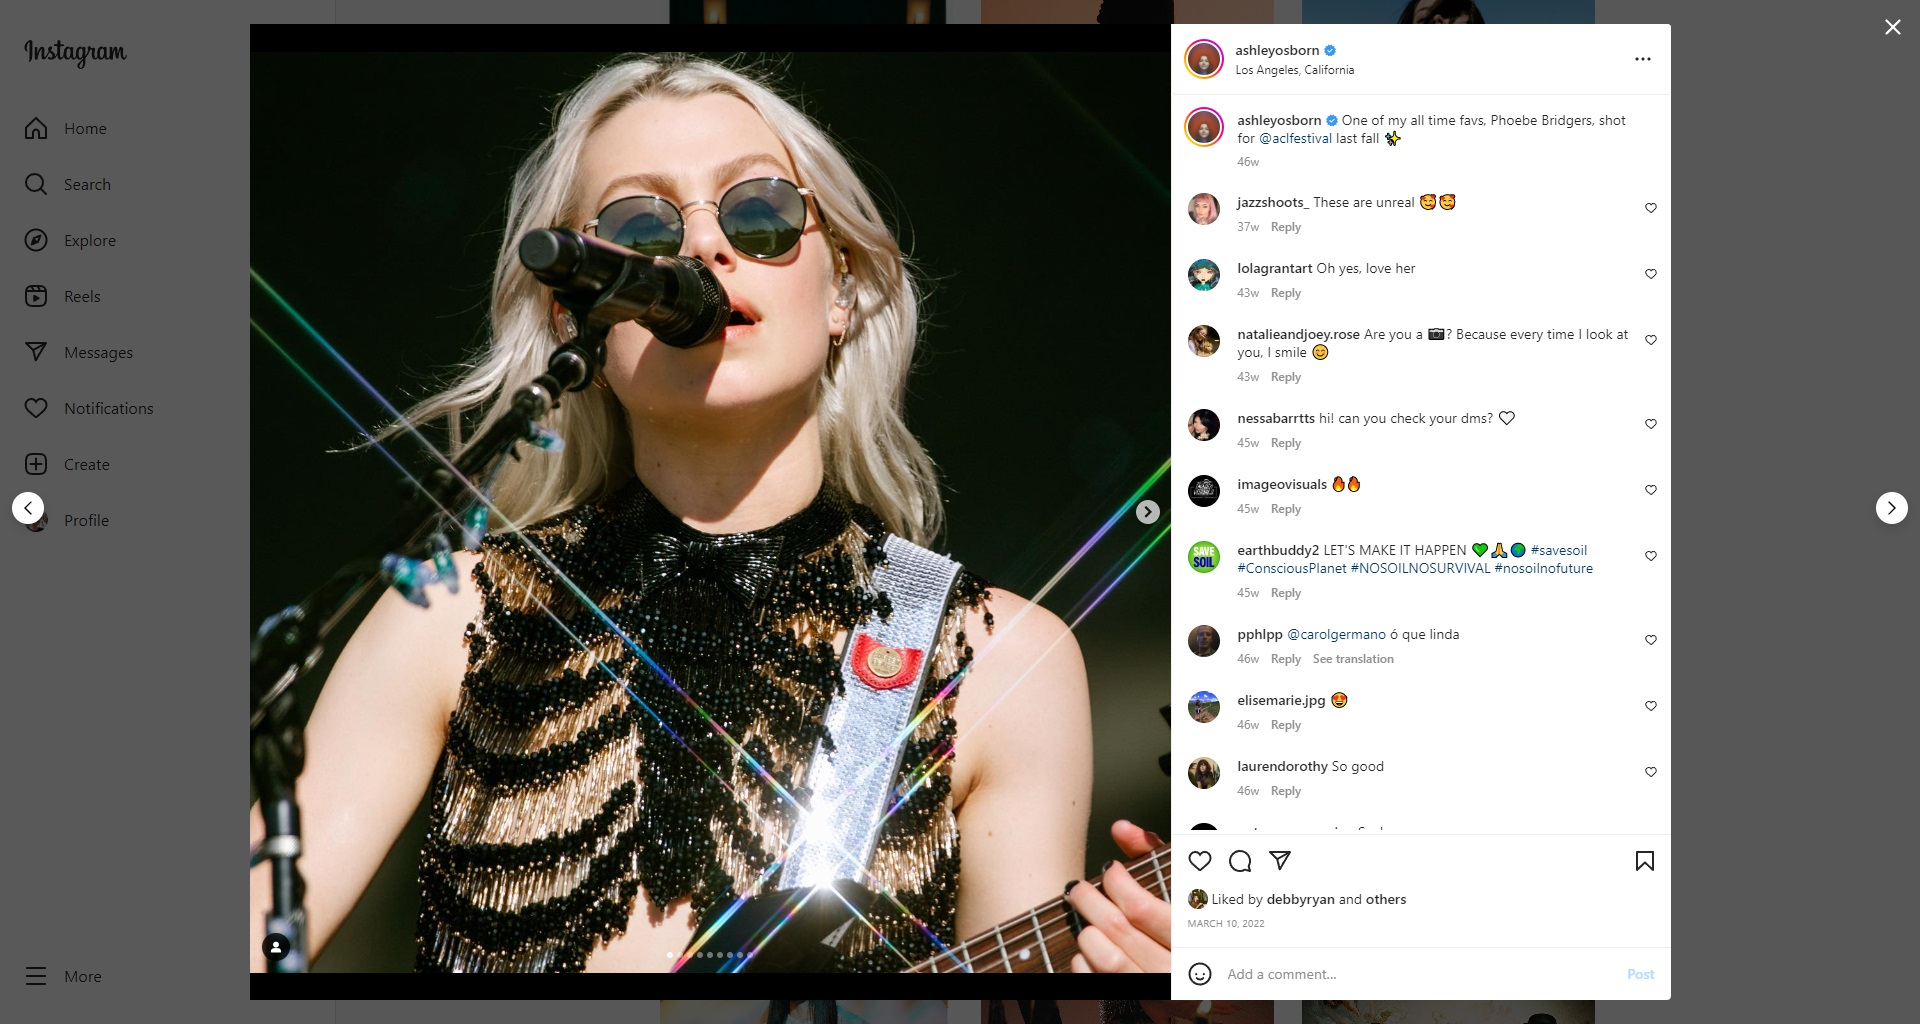
\includegraphics[width=0.95\textwidth]{images/instagram-2.jpg}}
   \caption{Instagram --- widok postu.}
   \label{fig:instagram-2.jpg}
\end{figure}

Kolejnym widokiem jest widok postu (rys. \ref{fig:instagram-2.jpg}). Pozwala on na przeglądanie wszystkich znajdujących się w nim filmów i zdjęć, czytanie i dodawanie komentarzy, polubienie postu oraz udostępnienie go za pomocą wiadomości prywatnej lub skopiowanie linku, aby umieścić go poza Instagramem. Warto zwrócić uwagę na przyciemnioną pozostałą część strony --- użytkownik po zamknięciu postu wróci do miejsca, od którego zaczął jego oglądanie. 

%%% Facebook

\subsubsection{Facebook}

Założony w 2004 roku \cite{historiafacebooka} Facebook to najpopularniejszy pod względem miesięcznej liczby użytkowników serwis społecznościowy \cite{socialmediastats}. Portal ten jest wykorzystywany zarówno do tworzenia profilów prywatnych, jak i firmowych. Użytkownicy mogą dodawać się nawzajem do grona znajomych, umieszczać na swojej tablicy posty tekstowe lub ze zdjęciami i filmami, tworzyć grupy, obserwować interesujące ich strony. Te ostatnie mogą reprezentować np. popularnych artystów, lokalne firmy lub po prostu umieszczać treści o określonej tematyce. Ze względu na ogromną popularność i idącym za nią potencjałem marketingowym posty publikowane przez strony mogą też być promowane, co zwiększa potencjalną liczbę odbiorców. Elementami profilu użytkownika są: 
\begin{itemize}
    \item część nagłówkowa zawierająca tło, zdjęcie profilowe, nazwę strony, liczbę osób obserwujących i obserwowanych, możliwość zaobserwowania profilu oraz opcję wyszukiwania (rys. \ref{fig:facebook-1.jpg});
    \item sekcja o nazwie ``Prezentacja'' --- krótki opis, informacja o rodzaju strony oraz odniesienie do strony internetowej (rys. \ref{fig:facebook-1.jpg});
    \item galeria zdjęć (rys. \ref{fig:facebook-2.jpg});
    \item uporządkowana chronologicznie (od najnowszego do najstarszego) lista postów (rys. \ref{fig:facebook-2.jpg}).
\end{itemize}
Posty mogą być wyświetlane oddzielnie. W zależności od tego, czy razem z nimi dodane jest zdjęcie lub film, widok ten się różni. Rysunek \ref{fig:facebook-3.jpg} przedstawia post ze zdjęciem, natomiast rysunek \ref{fig:facebook-4.jpg} --- post bez zdjęcia z osadzonym linkiem. Podobnie jak w przypadku strony prezentowanej \linebreak w podrozdziale \ref{ashley}, warto zwrócić uwagę na ograniczoną szerokość posta, a co za tym idzie --- tekstu, zwłaszcza na rysunku \ref{fig:facebook-4.jpg}. 

\begin{figure}[H] 
    \centering
         \fbox{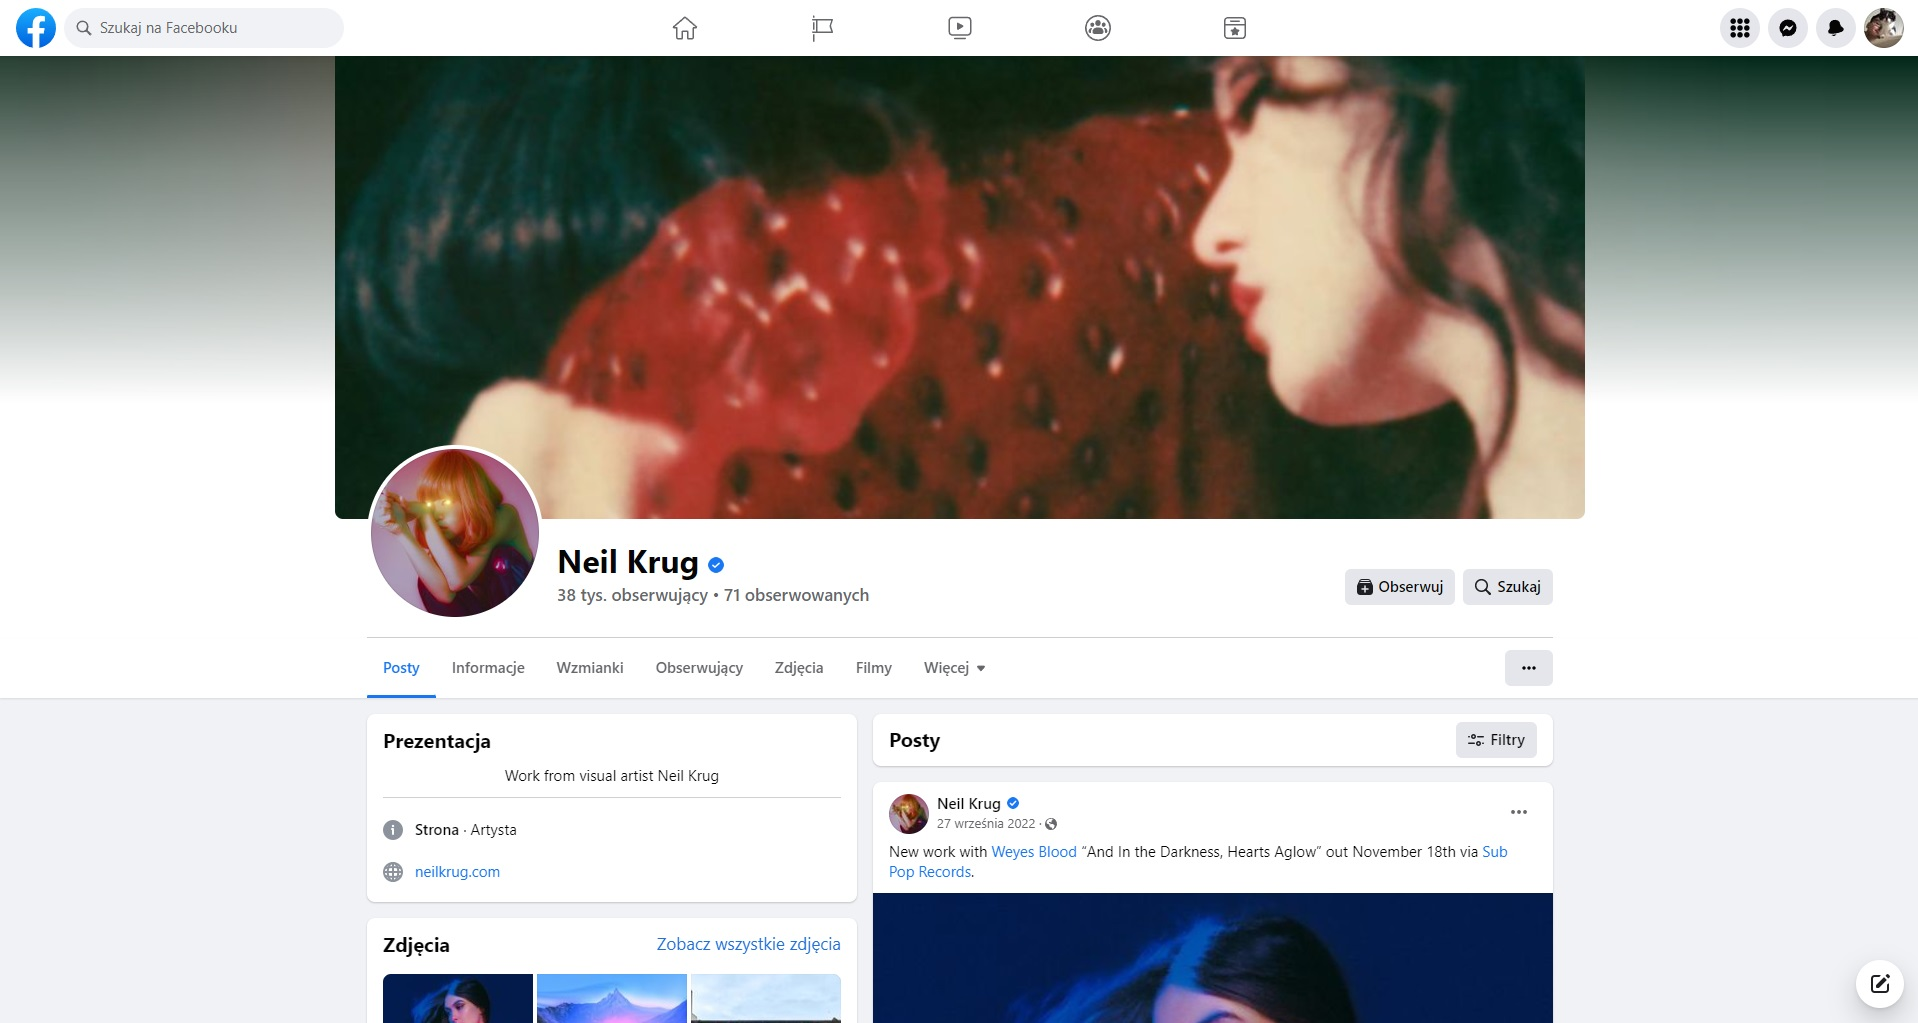
\includegraphics[width=0.99\textwidth]{images/facebook-1.jpg}}
   \caption{Facebook --- widok profilu użytkownika ze zdjęciem w tle.}
   \label{fig:facebook-1.jpg}
\end{figure}

\begin{figure}[H] 
    \centering
         \fbox{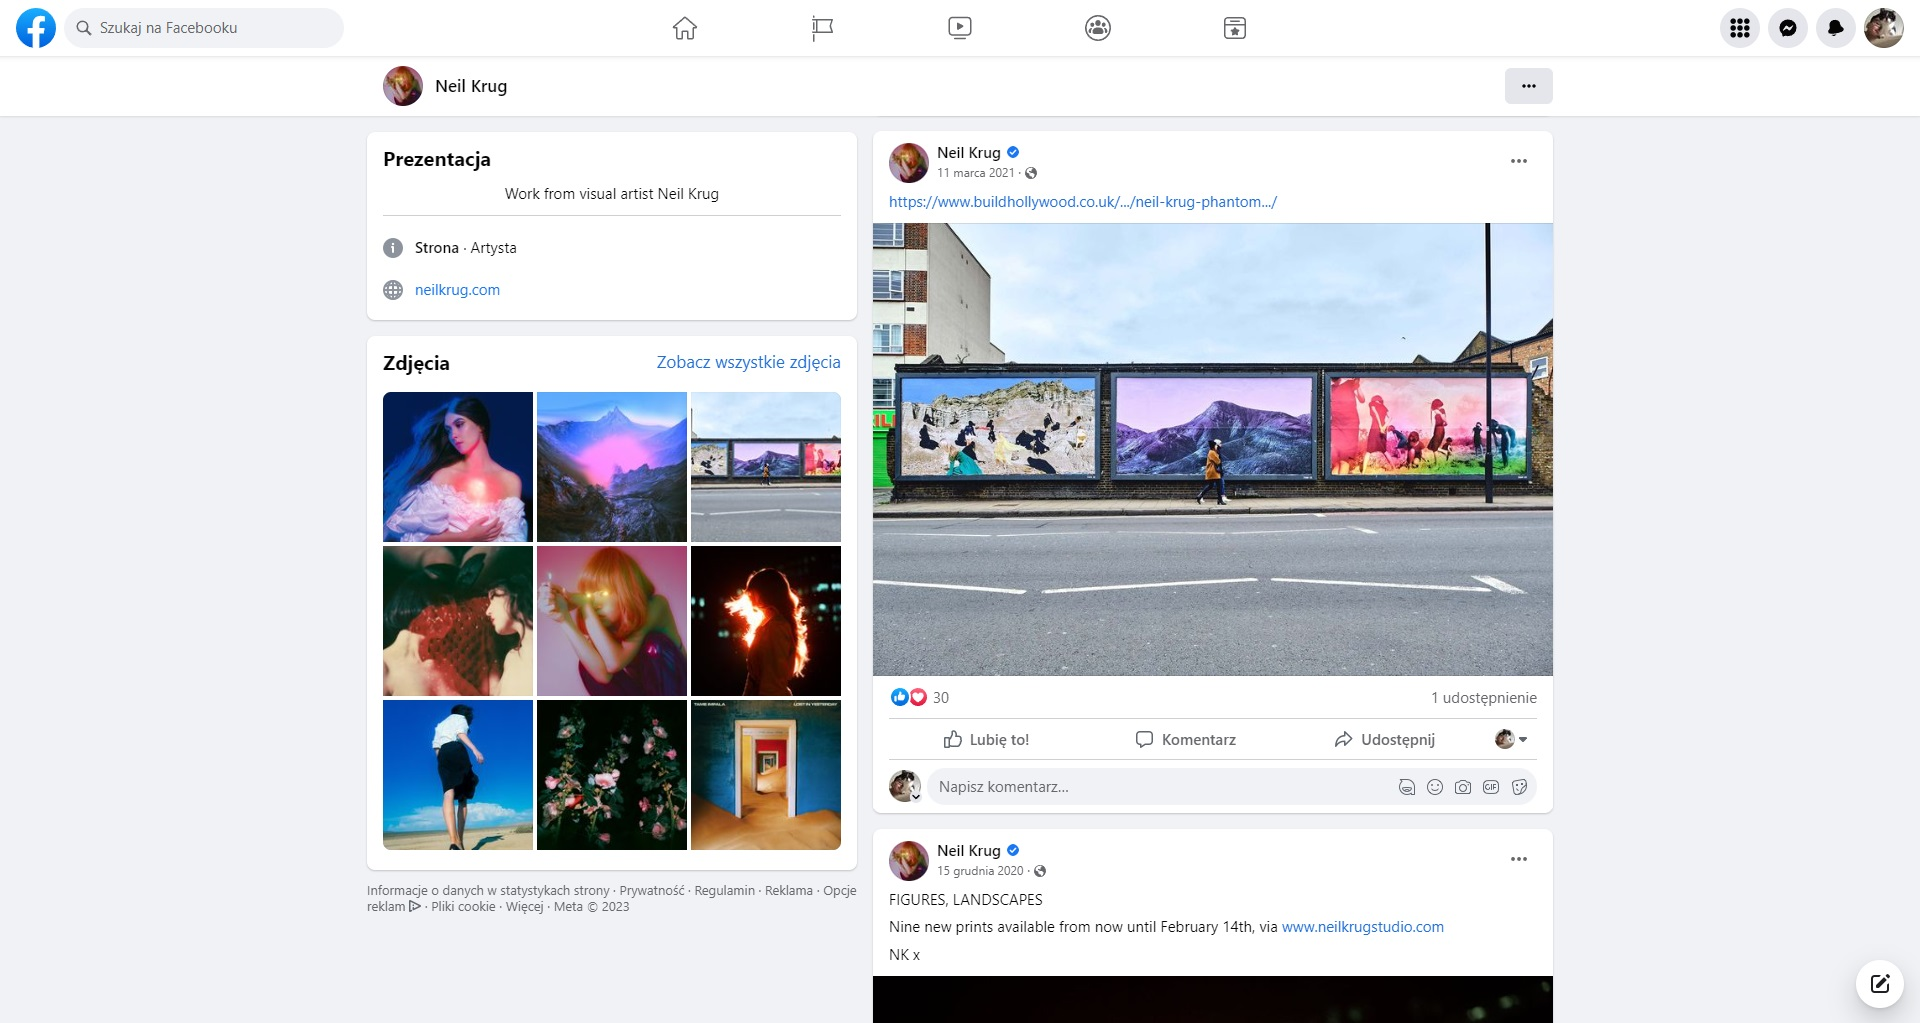
\includegraphics[width=0.99\textwidth]{images/facebook-2.jpg}}
   \caption{Facebook --- widok tablicy użytkownika po przewinięciu.}
   \label{fig:facebook-2.jpg}
\end{figure}

\begin{figure}[H] 
    \centering
         \fbox{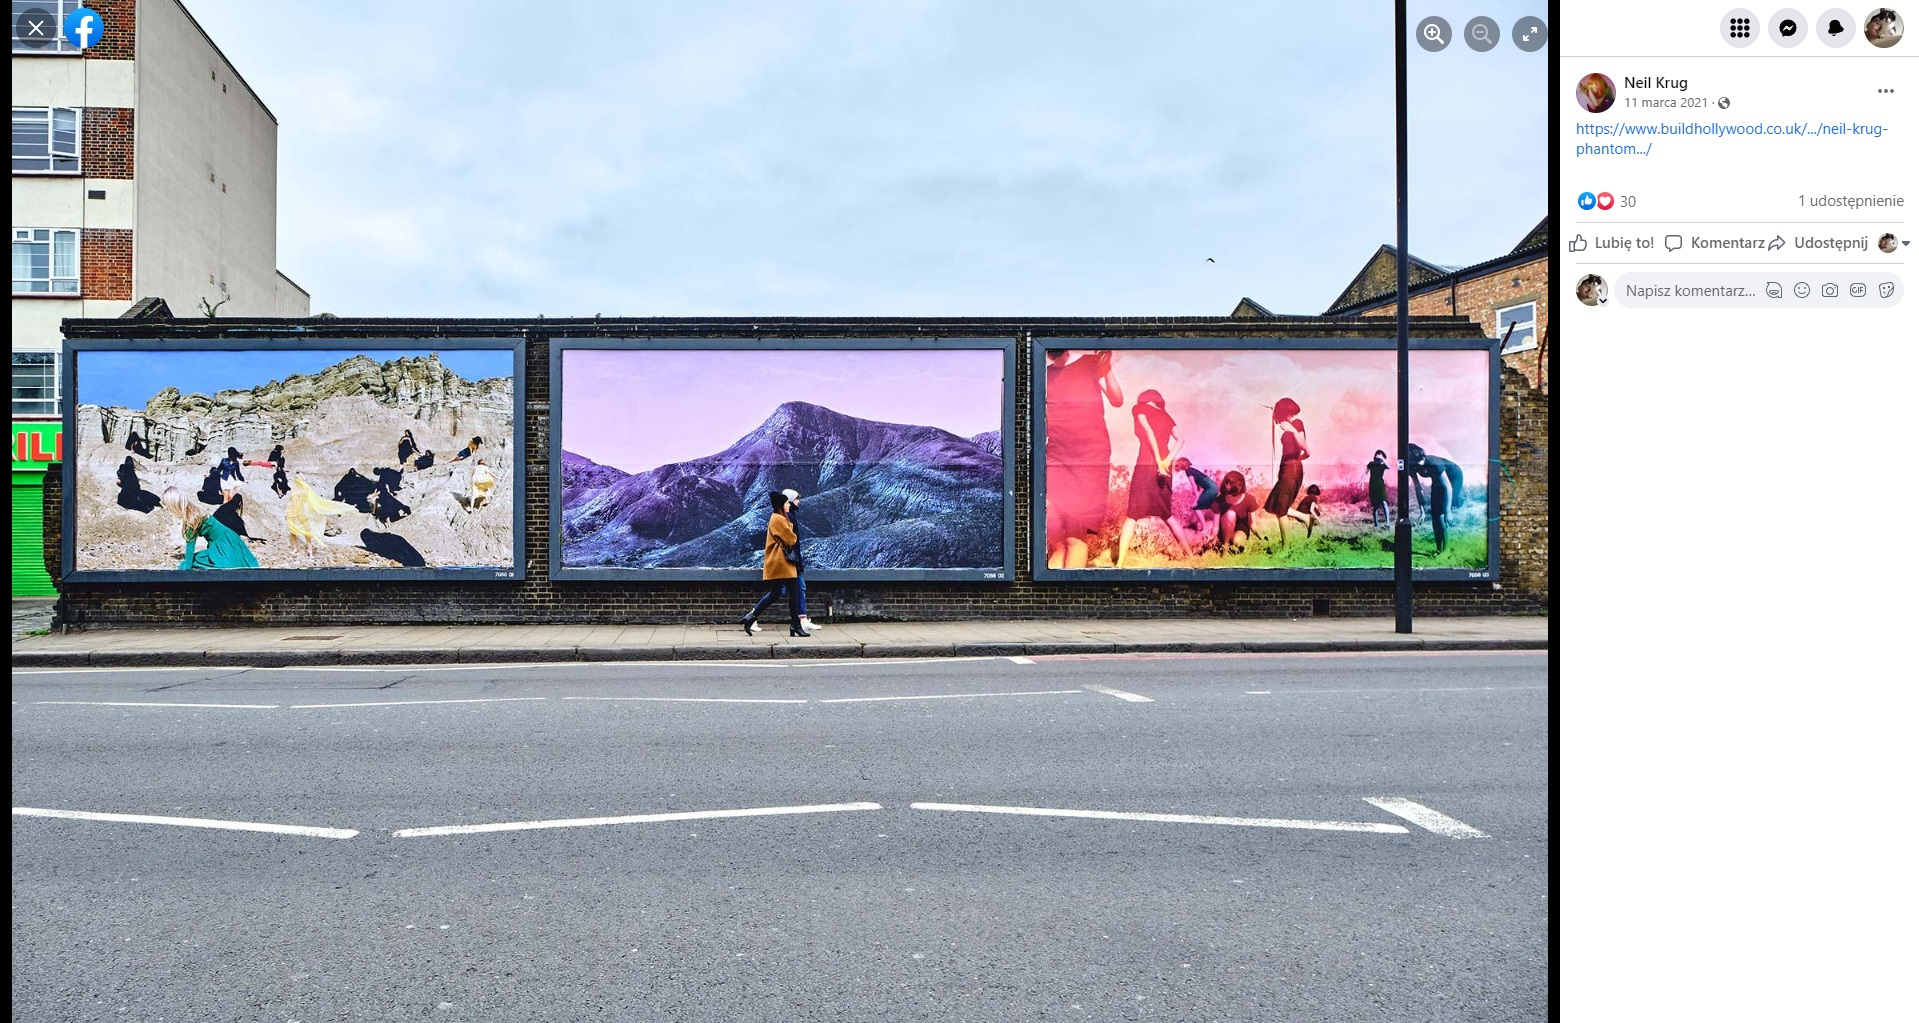
\includegraphics[width=0.99\textwidth]{images/facebook-3.jpg}}
   \caption{Facebook --- widok postu ze zdjęciem.}
   \label{fig:facebook-3.jpg}
\end{figure}

\begin{figure}[H] 
    \centering
         \fbox{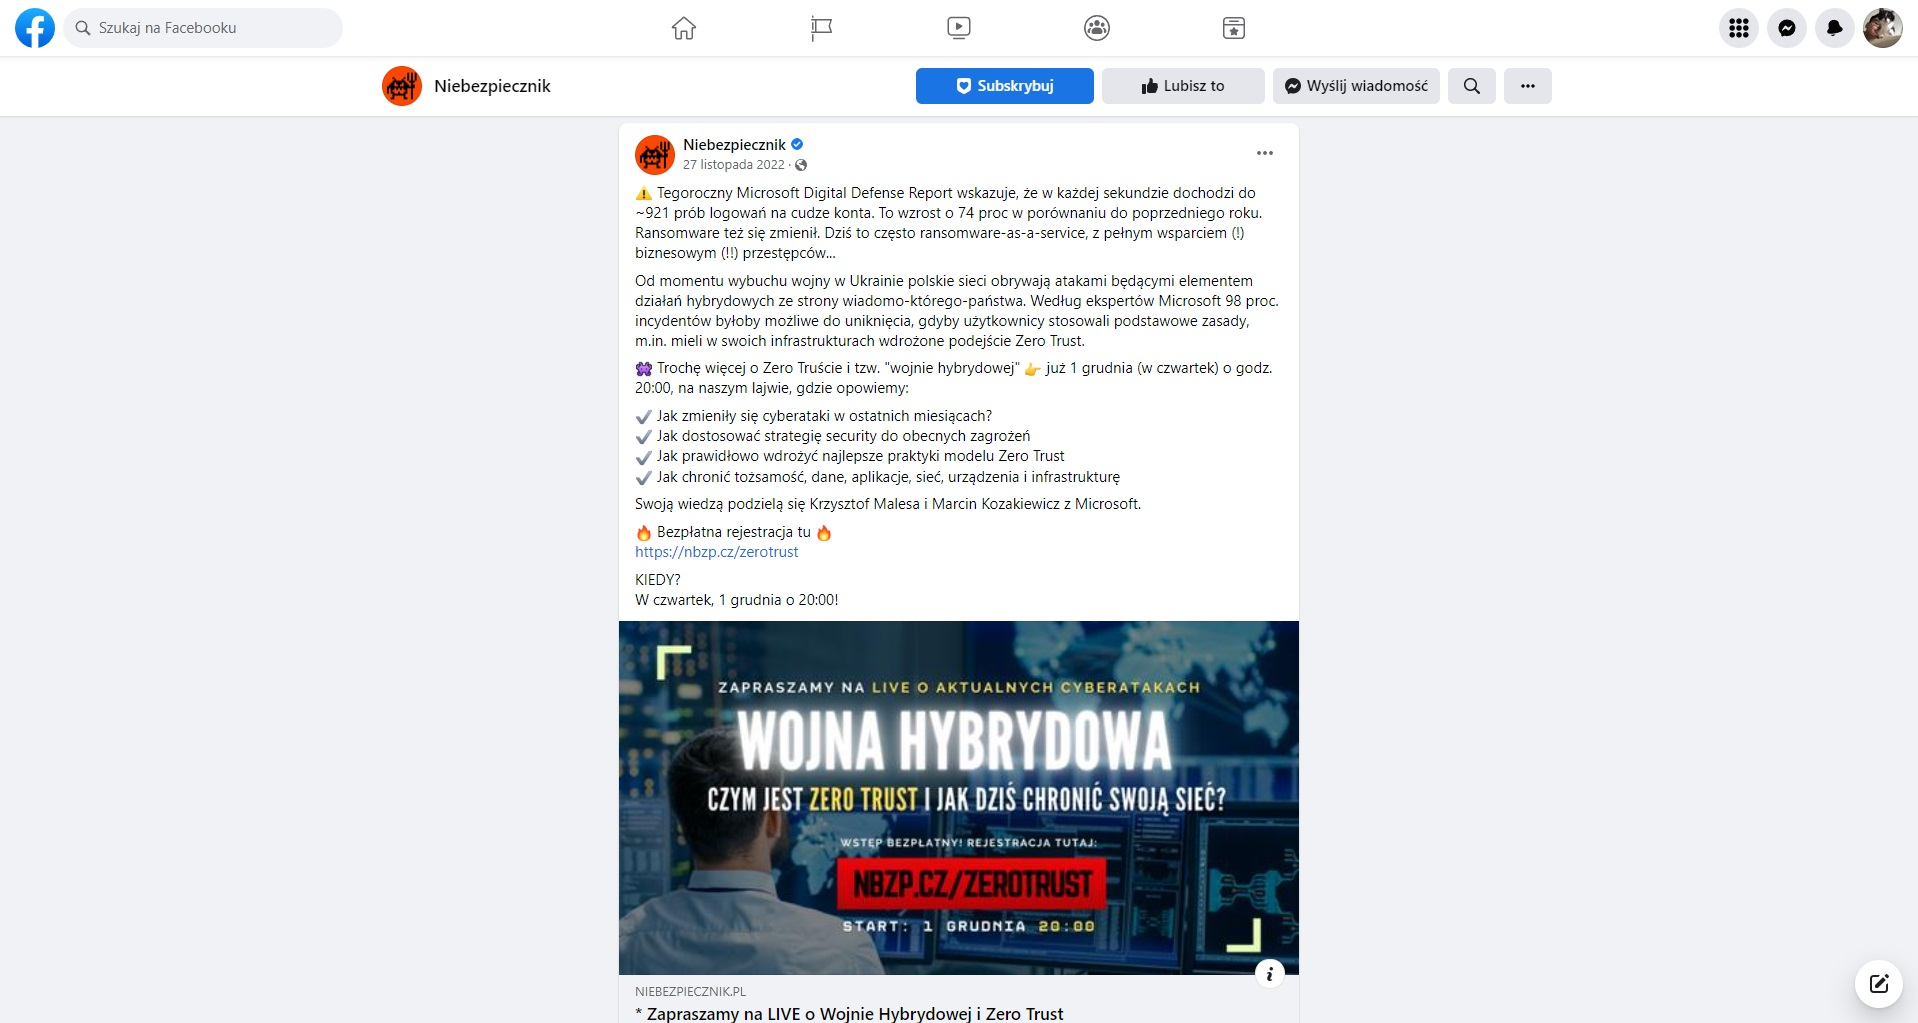
\includegraphics[width=0.99\textwidth]{images/facebook-4.jpg}}
   \caption{Facebook --- widok postu tekstowego (z osadzonym linkiem).}
   \label{fig:facebook-4.jpg}
\end{figure}

\subsection{Podsumowanie przeglądu}

Biorąc pod uwagę cechy analizowanych stron-wizytówek oraz portali społecznościowych używanych do pozyskiwania nowych klientów i promowania własnych prac, wyciągnięte zostały wnioski dotyczące podejścia do tworzenia projektu strony internetowej oraz planowania jej funkcjonalności. Po pierwsze, strony internetowe zawierające portfolio powinny być proste pod względem nawigacji (np. widoczny cały czas pasek nawigacyjny) oraz projektu graficznego (minimalistyczny układ i prosta kolorystyka pozwalają skupić się na treści). Po drugie, w przypadku występowania większej ilości tekstu, wskazane jest zachowanie ograniczonej szerokości bloku tekstu. Strona główna jest pierwszym miejscem, w które trafia użytkownik, więc przydadzą się na niej skupiające uwagę zdjęcia (może to być spektakularna sceneria, ale też na przykład ktoś sławny). Sekcja ``o mnie'' powinna natomiast zawierać zwięźle opisany życiorys oraz doświadczenie zawodowe. W przypadku obecności formularza kontaktowego należy pamiętać o walidacji wprowadzanych przez użytkownika danych oraz wyświetlaniu rezultatu próby wysłania danych. W czasach ogromnej popularności mediów społecznościowych dobrą praktyką jest też umieszczenie odnośników do znajdujących się tam profili fotografa.

% Narzędzia wybrane do realizacji projektu

\newpage 

\section{Narzędzia wybrane do realizacji projektu}

Niniejszy rozdział przedstawia narzędzia, które zostały wykorzystane do wykonania projektu graficznego tworzonej strony oraz jego realizacji. Ich wybór podyktowany był wcześniejszym doświadczeniem, dostępnością dokumentacji oraz dostosowaniem do wymagań projektowych, które zostały przedstawione w rozdziale \ref{wymagania}.

%% Figma

\subsection{Figma}
\begin{figure}[H] 
    \centering
         \fbox{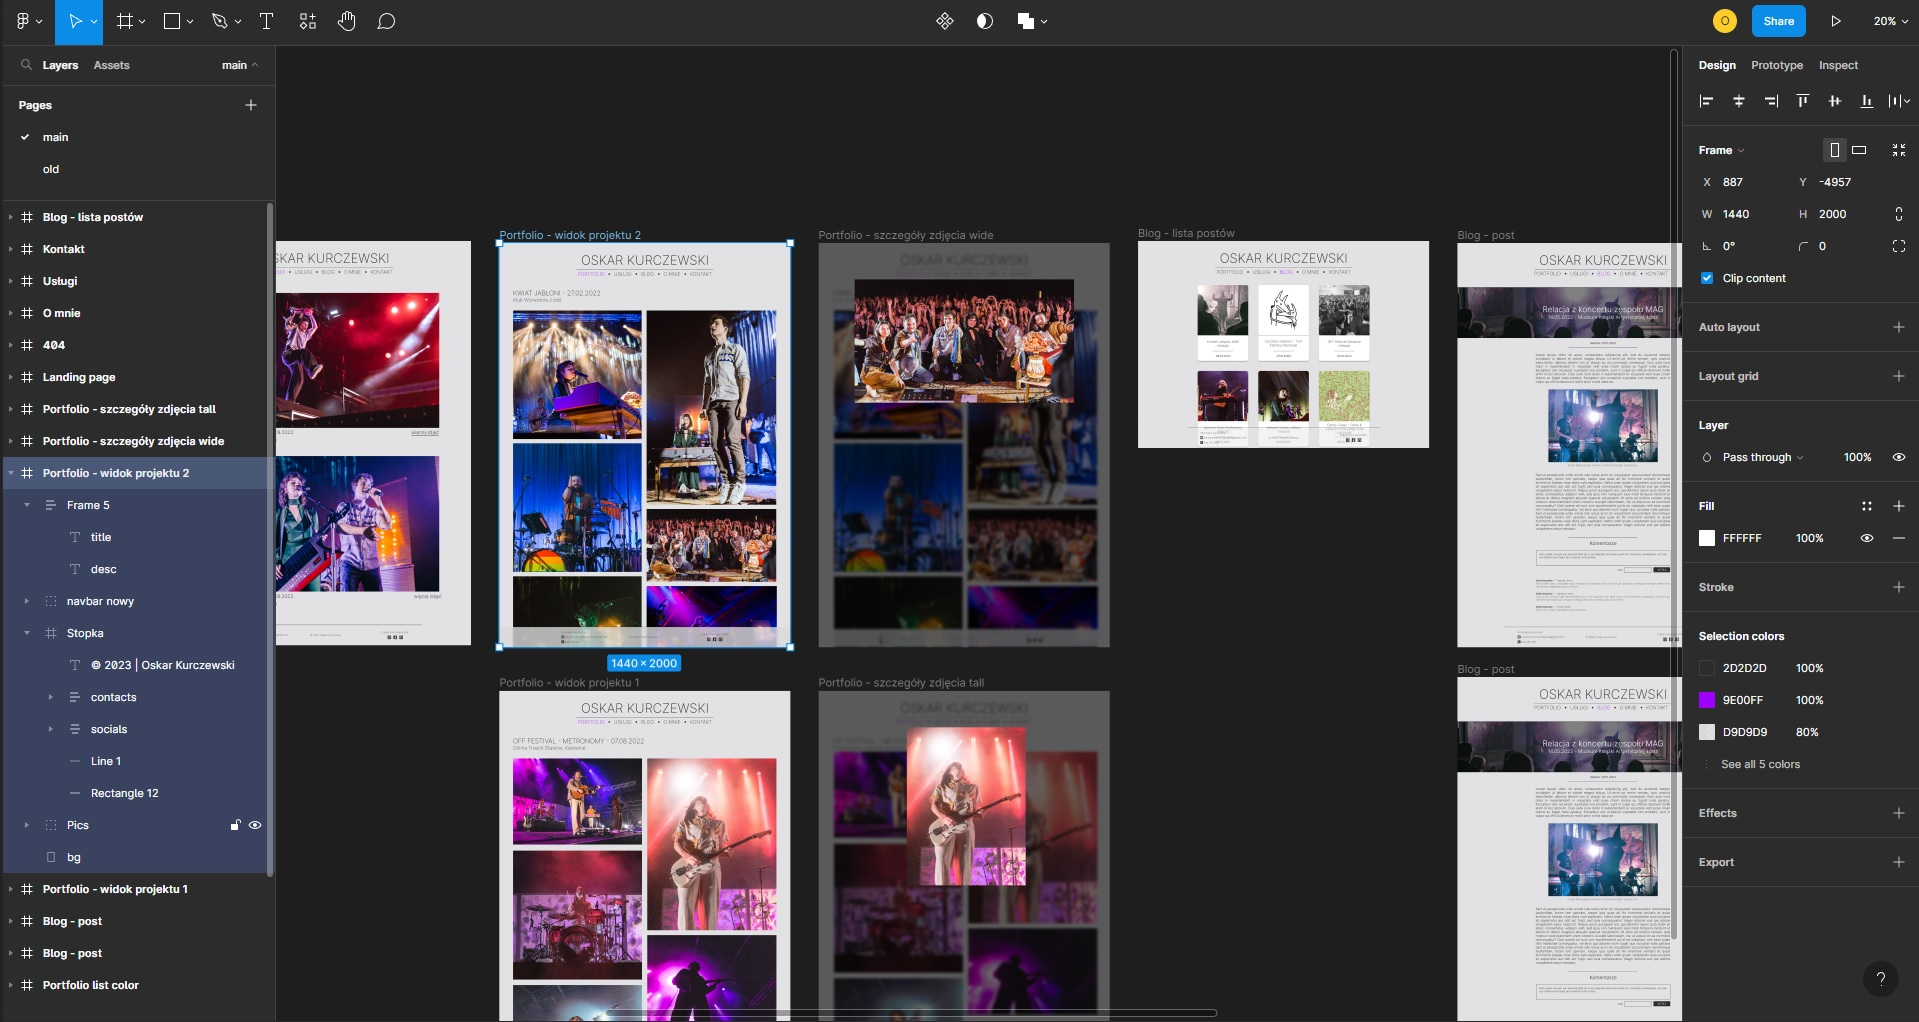
\includegraphics[width=0.99\textwidth]{images/figma-1.jpg}}
   \caption{Interfejs użytkownika narzędzia Figma.}
   \label{fig:figma-1.jpg}
\end{figure}

Wcześniejsze wykonanie projektu graficznego tworzonej strony internetowej pozwala na jej łatwiejszą implementację. Taki interfejs użytkownika jest też bardziej spójny wizualnie, co jest ważne dla pozytywnego odbioru strony. Do sporządzenia projektu strony-portfolio z blogiem wykorzystane zostało narzędzie Figma (rys. \ref{fig:figma-1.jpg}) --- prosty w obsłudze program pozwalający na wykonanie interaktywnych projektów interfejsów użytkownika za pomocą grafiki wektorowej \cite{figma}. 

%% JavaScript

\subsection{JavaScript}

Do implementacji tworzonego projektu wykorzystany został JavaScript (JS), czyli najpopularniejszy język programowania na świecie \cite{js}. Cechują go: wieloplatformowość, wysokopoziomowość i dynamiczne typowanie. Jako zaletę języka JavaScript można wymienić wsparcie dla wielu platform --- tworzone za jego pomocą aplikacje mogą być używane zarówno na urządzeniach mobilnych, jak i w przeglądarce. Ponadto duży wybór bibliotek oraz szkieletów aplikacyjnych ułatwia dobranie odpowiednich narzędzi do danego typu projektu.

%% Node/NPM

\subsection{Node.js oraz \textit{npm}}

Node.js to wieloplatformowe środowsko uruchomieniowe zbudowane w języku JavaScript \cite{node}. Jego działanie jest oparte na zdarzeniach asynchronicznych, dzięki czemu aplikacja stworzona w Node.js działa jako jeden proces. Integralnym elementem środowiska Node.js jest npm (Node Package Manager) --- system zarządzania pakietami pozwalający na łatwą instalację wybranych bibliotek i narzędzi \cite{npm}. 

%% Strapi

\subsection{Strapi}

Strapi to system zarządzania treścią (CMS) typu \textit{headless} --- oznacza to, że nie posiada on warstwy widoku, co daje dużą dowolność w zakresie doboru technologii odpowiedzialnej za wyświetlanie dodanych treści. Głównymi cechami Strapi są:
\begin{itemize}
    \item wsparcie dla wielu systemów zarządzania bazami danych --- SQLite (domyślny), MySQL, PostresQL oraz MariaDB \cite{strapifeatures};
    \item 
\end{itemize}

%% Next.js

\subsection{Next.js}

%% SCSS

\subsection{Sass (SCSS)}

Sass to preprocesor CSS 

% Projekt portfolio i blogu

\newpage 

\section{Projekt portfolio i blogu} \label{wymagania}

%% Założenia projektu

\subsection{Założenia projektu}

%% Wymagania funkcjonalne

\subsection{Wymagania funkcjonalne}

%% Wymagania niefunkcjonalne

\subsection{Wymagania niefunkcjonalne}


%% Realizacja projektu 

\subsection{Realizacja projektu}

% Portfolio i blog

\newpage

\section{Portfolio i blog}

%% System zarządzania treścią

\subsection{System zarządzania treścią}


%% Strona internetowa

\subsection{Strona internetowa}

% Podsumowanie

\newpage 

\section{Podsumowanie}

% Spis rysunków

\newpage 

\addcontentsline{toc}{section}{\protect\numberline{}Spis rysunków}%
    \listoffigures
    \clearpage

% Spis tabel

\newpage 

\addcontentsline{toc}{section}{\protect\numberline{}Spis tabel}%
    \listoftables
    \clearpage

% Spis listingów

\newpage 

\addcontentsline{toc}{section}{\protect\numberline{}Spis listingów}%
    \listofcodes
    \clearpage

% Bibliografia

\newpage 

\section*{Bibliografia}
    \addcontentsline{toc}{section}{\protect\numberline{}Bibliografia}%
    \renewcommand{\section}[2]{}
    
\begin{thebibliography}{99}

    \bibitem{fotografia}
    Leszek J. Pękalski,
    \textit{Kalejdoskop fotografii. Między techniką a sztuką},
    Helion,
    2012.

    \bibitem{nobelfoto} 
    The Nobel Prize in Physics 2009,
    \url{https://www.nobelprize.org/prizes/physics/2009/summary/}, 
    dostęp 27.01.2023.

    \bibitem{firstdigitalphoto}
    The first digital photos, National Science and Media Museum,
    \url{https://www.scienceandmediamuseum.org.uk/objects-and-stories/first-digital-photos},
    dostęp 27.01.2023.

    \bibitem{instagram}
    Most followers on Instagram, Statista,
    \url{https://www.statista.com/statistics/421169/most-followers-instagram/},
    dostęp 27.01.2023.

    \bibitem{socialmediastats}
    Global social networks ranked by number of users, Statista,
    \url{https://www.statista.com/statistics/272014/global-social-networks-ranked-by-number-of-users/},
    dostęp 27.01.2023

    \bibitem{ashley}
    Ashley Osborn,
    \url{https://www.ashleyosborn.com/},
    dostęp 27.01.2023.

    \bibitem{stateofphotography}
    State of the Photography Industry Report 2022, Format,
    \url{https://www.format.com/magazine/features/photography/state-of-the-photography-industry-2022},
    dostęp 27.01.2023.

    \bibitem{projektowanie}
    Jason Beaird, James George,
    \textit{Niezawodne zasady web designu. Projektowanie spektakularnych witryn internetowych. Wydanie III},
    Helion,
    2015.

    \bibitem{formularze}
    Jennifer Niederst Robbins,
    \textit{Projektowanie stron internetowych. Przewodnik dla początkujących webmasterów po HTML5, CSS3 i grafice. Wydanie IV},
    Helion,
    2014.

    \bibitem{szerokosc}
    Line Length Readability, Baymard,
    \url{https://baymard.com/blog/line-length-readability},
    dostęp 27.01.2023

    \bibitem{socialmedia}
    Marcin Żukowski,
    \textit{Twoja firma w social mediach. Podręcznik marketingu internetowego dla małych i średnich przedsiębiorstw},
    Helion,
    2016.

    \bibitem{figma}
    Fabio Staiano,
    \textit{Designing and Prototyping Interfaces with Figma},
    Packt Publishing,
    2022.

    \bibitem{js}
    David Flanagan,
    \textit{JavaScript. Przewodnik. Poznaj język mistrzów programowania. Wydanie VII},
    Helion,
    2021.

    \bibitem{historiafacebooka}
    Facebook Overview, History \& Facts, Britannica,
    \textit{https://www.britannica.com/topic/Facebook},
    dostęp 27.01.2023.

    \bibitem{stories}
    Introducing Instagram Stories,
    \textit{https://about.instagram.com/blog/announcements/introducing-instagram-stories},
    dostęp 27.01.2023.

    \bibitem{instagramfirstday}
    A Brief History of Instagram's Fateful First Day, Time,
    \textit{https://time.com/4408374/instagram-anniversary/},
    dostęp 27.01.2023.

    \bibitem{strapidocs}
    Strapi Developer Docs,
    \textit{https://docs.strapi.io/developer-docs/latest/getting-started/introduction.html},
    dostęp 27.01.2023.

    \bibitem{strapifeatures}
    Strapi Features,
    \textit{https://strapi.io/features},
    dostęp 27.01.2023.

    \bibitem{node}
    About Node.js,
    \textit{https://nodejs.org/en/about/},
    dostęp 27.01.2023.

    \bibitem{npm}
    About npm,
    \textit{https://www.npmjs.com/about},
    dostęp 27.01.2023.
        
\end{thebibliography}

\end{sloppypar}
\end{document}